\documentclass[sigconf,manuscript,review,anonymous]{acmart} %Add anonymous next to sigconf to remove author information. Two column format is [sigconf]


%\settopmatter{printacmref=false} % Removes citation information below abstract

%\renewcommand\footnotetextcopyrightpermission[1]{} % removes footnote with conference information in first column

%Added for word count
%TC:macro \cite [option:text,text]
%TC:macro \citep [option:text,text]
%TC:macro \citet [option:text,text]
%TC:envir table 0 1
%TC:envir table* 0 1
%TC:envir tabular [ignore] word
%TC:envir displaymath 0 word
%TC:envir math 0 word
%TC:envir comment 0 0
\def\ts{TIPP\&SEE}
\def\cvd{COVID-19}
\def\umc{Use\begin{math}\rightarrow\end{math}Modify\begin{math}\rightarrow\end{math}Create\ }
\def\um{Use\begin{math}\rightarrow\end{math}Modify\ }
\pagestyle{plain} % removes running headers

\usepackage{color}
\usepackage{balance}
\usepackage{caption}
\usepackage{subcaption}
\usepackage{nicematrix}
\usepackage{multirow}
\usepackage{multicol}
\usepackage{graphicx}

\newcommand{\jen}[1]{\textcolor{red}{\textit{Jen: #1}}}
\newcommand{\diana}[1]{\textcolor{blue}{\textit{Diana: #1}}}
\newcommand{\merijke}[1]{\textcolor{purple}{\textit{Merijke: #1}}}
\newcommand{\donna}[1]{\textcolor{green}{\textit{Donna: #1}}}
\newcommand{\pratham}[1]{\textcolor{orange}{\textit{Pratham: #1}}}
\newcommand{\elizabeth}[1]{\textcolor{olive}{\textit{Elizabeth: #1}}}
\newcommand{\jean}[1]{\textcolor{violet}{\textit{Jean: #1}}}
\newcommand{\ourcomment}[1]{}
\newcommand{\hide}[1]{}
\fancyhead{}

\newcommand{\Scratchencore}[0]{Blinded Curriculum}
%\newcommand{\Scratchencore}[0]{Scratch Encore}

\usepackage{booktabs,verbatim} % For formal tables
%\usepackage[backend=bibtex,
%style=numeric,
%bibencoding=ascii
%style=alphabetic
%style=reading
%]{biblatex}
%\addbibresource{ref.bib}

\graphicspath{{images/}}

% Copyright
%\setcopyright{none}
%\setcopyright{acmcopyright}
%\setcopyright{acmlicensed}
%\setcopyright{rightsretained}
%\setcopyright{usgov}
%\setcopyright{usgovmixed}
%\setcopyright{cagov}
%\setcopyright{cagovmixed}

%Conference; not necessary for AERA
\copyrightyear{2021}
\acmYear{2021}
\setcopyright{acmcopyright}
\acmConference[ICER '20]{Proceedings of the 2020 International Computing Education Research Conference}{August 10--12, 2021}{Virtual Event, Toronto}
\acmBooktitle{Proceedings of the 2021 International Computing Education Research Conference (ICER '21), August 10--12, 2021, Virtual Event, Toronto, Canada}
\acmPrice{15.00}
\acmDOI{10.1145/3372782.3406256}
\acmISBN{978-1-4503-7092-9/20/08}

\settopmatter{printacmref=false, printfolios=false}

\begin{document}
\title[]{Comparison of CS Instruction during Pre-Pandemic, Pandemic and Post-Pandemic{} School Years}

\author{David A. Gonzalez-Maldonado$^\dagger$, Donna Eatinger$^\ast$, Diana Franklin$^\ast$, Pratham Gandhi$^\ast$, Jennifer Palmer$^\ast$, Elizabeth N. Singer$^\ast$, Jean Salac$^\ast$, Jennifer Tsan$^\ast$,David Weintrop$^\dagger$}
\affiliation{%
  \institution{$^\ast$University of Chicago, Chicago, IL, USA \\
  $^\dagger$ University of Maryland, College Park, College Park, MD, USA \\
    %$^\ddagger$ Chicago Public Schools, Chicago, IL, USA 
    }
}
\email{{dagm,dmeatinger,dmfranklin,pratham,jenpalmer,ensinger,salac,jennifertsan}@uchicago.edu; {mcoenraa, weintrop}@umd.edu
}

\pagenumbering{gobble}

\begin{abstract}
% As computer science (CS) instruction matures at the elementary and middle-school levels, new pedagogical approaches, learning strategies, and teaching strategies are being developed. Because of the great increase in development between 4th grade (ages 9-10) and 7th grade (ages 12-13), students may respond differently to the same approach. In this paper, we explore middle-grade students' (age 9-13, grades 4-7) use of \ts{} in an intermediate, Scratch-based, \umc programming curriculum. \Scratchencore{} was designed to be an intermediate programming curriculum. %and studied with 4th grade students.
% We present analysis of 307 students' work, investigating student participation and accuracy in the different \ts{} phases. Our findings show that middle-grade students who use \ts{} show similar engagement and answer questions with the similar correctness across a variety of factors such as previous experience with programming (parent-reported). However, among the \ts{} phases, the students demonstrated higher engagement and the most success with answering questions that involve observing an example program operation before (``Observe'') or after making changes to the program (``Explore'') than with questions that involve making predictions about how the code may operate (``Predict''). We also found that students have the highest engagement and accuracy when answering questions about concepts that could have an every-day interpretation, such as the \texttt{say} block. Finally, our results show that student engagement and correctness for a given question is impacted by its placement on the worksheet. These findings reveal important design aspects of \ts{} and how it supports students across a variety of factors, and how students struggle with making ``Predictions'' and interpreting certain concepts correctly.

\end{abstract}

\begin{CCSXML}
<ccs2012>
<concept>
<concept_id>10003456.10003457.10003527.10003531.10003533</concept_id>
<concept_desc>Social and professional topics~Computer science education</concept_desc>
<concept_significance>500</concept_significance>
</concept>
<concept>
<concept_id>10003456.10003457.10003527.10003528</concept_id>
<concept_desc>Social and professional topics~Computational thinking</concept_desc>
<concept_significance>300</concept_significance>
</concept>
<concept>
<concept_id>10003456.10003457.10003527.10003541</concept_id>
<concept_desc>Social and professional topics~K-12 education</concept_desc>
<concept_significance>300</concept_significance>
</concept>
</ccs2012>
\end{CCSXML}
\ccsdesc[500]{Social and professional topics~Computer science education}

\acmPrice{15.00}

\keywords{Computational Science Education; K-12 education; Scratch}

\maketitle

%\setcopyright{acmcopyright}
{\fontsize{8pt}{8pt} \selectfont
\textbf{ACM Reference Format:} \\
%, Merijke Coenraad, Jennifer Palmer, Donna Eatinger,
%David Weintrop, Diana Franklin. 2020. 
An Analysis of Middle-School Student Behavior using the \ts{} Metacognitive Learning Strategy. In \textit{Proceedings
of the 2021 International Computing Education Research Conference (ICER’21), August 10–12, 2021, Virtual Event, Toronto, Canada.} ACM, New York, NY, USA, 11 pages. \ }

\section{Introduction}
\label{sec:objectives}

% Equitable and accessible instruction in computer science (CS) and computing is essential for preparing all students to succeed in an increasingly computationally-driven world. It is important that educational opportunities are not only available, but that students develop meaningful and actionable computing knowledge as part of this instruction. While much emphasis has been placed on the creation of introductory CS educational resources and computing courses in high school and higher education, there has been a gap in resources and computing courses for younger students. %Standardized CS coursework was first introduced in high schools in the United States in 1984 in the form of Advanced Placement courses which were created to provide college-level CS curricula and assessments to high schools students ~\cite{nageradamsatkinsonrobert, braswell1984advanced,apstudents}. As interest in creating CS curricula for younger students grew, resources and organizations like Code.org, founded in 2013, arose and offered introductory CS education to younger students ~\cite{codedotorgabout}. However,
% A study of curricula available to elementary and middle-school students in 2 regions of the United States showed a lack of specification of general purpose programming, object oriented programming, and visual programming \cite{falkner2019international}. In response to these and other gaps in instructional materials, \Scratchencore{} was designed to focus on elementary and middle-school students ~\cite{authors}. \Scratchencore{} employs a number of pedagogical innovations, including \ts{} which has been shown to promote students writing longer programs, writing more code per requirement, using more required blocks in later assignments, and satisfying more assignment requirements ~\cite{10.1145/3372782.3406257}. Overall, \ts{} has been shown to increase elementary-school student acquisition of computational knowledge, regardless of background and create more equitable access points for students ~\cite{10.1145/3372782.3406257}. In this paper, we explore the ways in which \emph{middle-grade students} interact with the \ts{} pedagogical strategy and if \ts{} supports their acquisition of computing knowledge. In order to understand the ways in which middle-grade students engage with \ts{}, in this paper, we address the following 3 research questions: 
% \begin{itemize}
% %\item How are students' responses and student engagement with \ts{} similar and how do they vary across the 3 sections of \ts{} -- Play, SE, and Explore?
% \item What level of completion and accuracy do middle-grade (4th-7th) students achieve across the 3 sections of \ts{}?
% \item What factors influence accuracy and completion rates of individual questions?
% %\item Is there any correlation between performance on \ts{} questions and other related learning activities?
% \item How do these findings compare with prior research on \ts{} with younger (4th grade) students?
% %\item Across sections of \ts{}, how does a problem's wording and connection to student prior knowledge affect student engagement?
% %\item How does \ts{} worksheet arrangement affect student behavior and scores?
% %\item In situations where student behavior and engagement in \ts{} differ greatly, what is the cause of these differences?
% %\item Is there a difference in student outcomes based on parent-reported student mathematics struggles or previous experience with programming?
% %\item How does the \ts{} strategy impact the work students produce later in the curriculum?
% \end{itemize}
% %^this last question is referring to Modify and Create scores
% This paper is organized as follows. In Section 2, we discuss the major theoretical and practical influences that inform this work. In Section 3, we describe the \ts{} strategy that scaffolds student development through the \um components of the \umc learning framework. Section 4 presents the methodological approach used to investigate the stated research questions. In Section 5, we present the main results of this paper, including overall performance and student-related, classroom-related, and question-related factors that affect student outcomes. In Section 6, we discuss these results relative to related work. The paper concludes with a review of the limitations of our findings and discussion of next steps for this work.

\section{Theory and Prior Work}
\label{sec:background}
\thispagestyle{empty}

% In this section, we present the major theoretical and practical influences that shaped this work. This includes prior work on theories concerning learning, teaching strategies, and middle-grade computing education curricula and pedagogy.

% \subsection{Theoretical Orientation}
% This work draws on constructionist learning theory and the concepts of the \textit{Zone of Proximal Development} (ZPD) and \textit{instructional scaffolding}. Constructionist learning theory focuses on developing opportunities for learners to construct their own knowledge, rather than the focusing on directly transmitting this knowledge to students through direct instruction \cite{Papert:1980}. Constructionist activities place students in project-based learning activities so they can learn through connecting what they already know to discoveries they make in the process of creating artifacts of their own \cite{papert1991situating, papert1993children}. Allowing students the freedom to construct their own understanding can lead to a number of challenges when employed in formal education contexts, such as keeping students on the intended learning trajectory and ensuring they learn specific content. In this process, some students may never reach the conclusions necessary or achieve the learning objectives of the activity. This tension between learner agency and externally defined learning goals, called the \textit{play paradox}, highlights the need for a strategy to support student exploration under sufficient constraints to ensure that specific learning outcomes are achieved \cite{noss1996windows}.

% The zone of proximal development describes the link between a student’s current abilities and their potential developmental achievements that can be attained through the guidance and encouragement from another, more skilled student \cite{vygotsky1980mind}. By providing further challenges to some students and through the use of instructional scaffolding— individualized support from the instructor that will be gradually removed— to others, the instructor can leverage each activity to keep students within their ZPD. This approach both maintains every student’s engagement and supports their individualized learning growth \cite{nasir2006, wood1976role}.

% The \umc educational framework combines constructionist learning theory, the ZPD, and instructional scaffolding as a strategy to avoid the play paradox \cite{lee2011computational, franklin2020analysis}. This approach involves students who are given constraints within which they can explore larger computing concepts, through modifying (within these constraints) a given code base. \umc initiates the learning experience with students in the Use activity, which provides examples of the focal concept being used and involves heavy scaffolding. The Modify activity follows with some of the scaffolds faded away as the students experience a guided exploration to modify the use of the concept. Students can then more directly explore the skills they have learned in a more powerful environment than their present skill level may support, but in a manner that enables them to gain intellectual ownership in this broader context. Finally, the Create activity allows them to explore and play, employing the concepts in ways they invent. This strategy increases students’ feeling of ownership over their work and appreciation for the context in which it lies in the broader computing framework \cite{lee2011, lytle2019use}.

% \subsection{Pedagogy In middle-grade Computing Education}

% Early access to computing education promotes equity and learning outcomes for computing education \cite{harel1990, Papert:1980, Papert:1979}. There is a wide array of computing curricula for elementary and middle-school students, including those based on structured, behaviorist curricula and direct instruction. On the other side of this spectrum are curricula that employ strategies to facilitate constructionist learning. This open-ended, student-centered approach allows students to discover the utility of each coding concept as they can be used in many situations, while gaining confidence in their abilities through feeling intellectual ownership over their own project. \cite{papert1993children, papert1991situating}. Most computing curricula and programming environments created for middle-grade students are based on constructionist or constructionist-inspired methods. While direct instruction may produce quicker learning outcomes in terms of student familiarity with specific learning objectives, constructionism promotes student engagement and confidence as they encourage students to create programming projects that they are excited about and proud to share with the world. \cite{brennan2012new, 10.1145/1345375.1345438} Many of these constructionist learning environments and curricula can trace their roots back to the Epistemology and Learning research group at MIT, including Logo, Scratch, NetLogo, and Lego Mindstorms. \cite{tippnsee, franklin2020Scratchencore}. These are also examples of the growing movement of block-based programming environments created to be accessible to students at all levels of prior computing knowledge. The drag-and-drop block-based format functions as scaffolding for students removing the potential for syntax errors and providing visual cues that are more approachable and similar to online games with which students new to programming may have more familiarity. \cite{Weintrop:2019, weintrop2017blockly, Weintrop:2015} Centered in the spectrum of computing curricula is the \umc framework.

% \subsection{Meta-cognitive Learning Strategies}

% \ts{} is a metacognitive learning strategy that proceduralizes student engagement to scaffold student learning (while learning from provided code as an example) and improves learning in the \um step of the \umc pedagogical approach designed for elementary computing instruction. \ts{} is based on reading comprehension strategies \cite{salac2020tippnsee}. Learning strategies are techniques, principles, and rules that teach students how to learn instead of teaching them specific content. These strategies enable students to learn, solve problems, and complete tasks independently \cite{deshler1986learning}. Meta-cognitive learning strategies in particular enable students to guide themselves through the learning process via a focus on self-regulation and self-motivation \cite{paris1990metacognition}. Students who use meta-cognition have knowledge and awareness about their own thinking, and are able to use this to bolster their learning by applying domain-appropriate learning strategies \cite{donker2014effectiveness}. Employing meta-cognitive strategies results in students having improved memory, test scores, and lecture comprehension \cite{king1991improving, kramarski2002effects}. 

% %As defined by Pressley et al. \cite{pressley2010cognitive}, these ``Good Strategy Users'' (GSU) have: 1) many learning techniques to draw from, 2) an understanding of when particular techniques are most applicable, 3) a recognition that increased effort leads to increased performance (and that distractions and other competing behaviors detract from effort), and 4) domain-specific knowledge which improves the efficiency of strategy deployment.

% The motivation behind explicitly teaching meta-cognition is that behaviors of students who naturally use meta-cognitive strategies are intrinsic to the students themselves, and thus non-meta-cognitive learners are further disadvantaged when not taught the process of learning \cite{cubukcu2008enhancing}. Thus, to create more equitable learning environments, hidden meta-cognitive behaviors have to be revealed to all learners by teaching meta-cognitive learning strategies. Mnemonic devices are one such meta-cognitive strategy. Mnemonic devices use acronyms to scaffold meta-cognition by prompting lists of information or actions comprising learning strategies \cite{scruggs2010mnemonic}. Mnemonic devices are often used along with other meta-cognitive learning strategies for reading comprehension, such as Previewing and Text Structure. Previewing guides students to identify important sections of text and call on related previous knowledge before reading. Text Structure prompts students to recognize the underlying organization of a text and retrieve structure-relevant processing strategies, thus enhancing their comprehension \cite{gersten2001teaching}. Teaching such comprehension strategies to middle-grade students in particular has been shown to improve performance on text summarizing, comprehension, memory, and maintenance of performance gains over time \cite{brown1984instructing}. Researchers have thus explored deploying comprehension strategies to create equitable learning opportunities in areas such as mathematics \cite{montague1992effects}, writing \cite{graham2012meta}, history \cite{de2005effects}, and most recently, CS \cite{franklin2020Scratchencore, salac2020tippnsee}.

% Within CS, comprehension strategies are especially crucial in enabling students' comprehension of code throughout a programming assignment, as they are required to read and process text such as individual instructions, sequences of instructions in the form of example code, and their own partially or fully complete code \cite{tippnsee}. Indeed, the aforementioned examples of comprehension strategies can aid in this. When Previewing, students can identify familiar and new code, connect unfamiliar concepts to prior knowledge, and use that to guess how the new code functions. Using Text Structures to understand the structure of the specific programming language and environment in which the students are working will allow them to draw on particular strategies for that scenario. 

% Researchers have shown that successful CS students also employ meta-cognitive comprehension strategies such as self-assessing understanding, creating timelines to track progress, and actively troubleshooting issues \cite{rum2018strategies}. Work on one specific CS comprehension strategy, \ts{}, has demonstrated that upper elementary-school aged students using the strategy have a more sophisticated understanding of CS concepts and increased performance on moderate to hard questions \cite{tippnsee}. This strategy is presented in more detail in the following section.

% The researchers who introduced \ts{} conducted an experimental study that showed that \ts{} improves performance in assessment questions and tasks in which the students were asked to explain scripts in their own words and make predictions. The students who used \ts{} outperformed the control students who used an unmodified \umc approach on almost every moderate and hard question. The researchers concluded that the additional scaffolding offered by \ts{} promotes better, deeper, and more sophisticated understanding of the introductory concepts for which it was used to learn (in this case events, sequence, loops) especially for advanced questions ~\cite{salac2020tippnsee}.

% Prior work analyzed student artifacts, assessments, and \ts{} worksheets and found that students who use \ts{} are more thorough in their work, write longer scripts, use more learned blocks, and are more accurate in their question responses. The researchers concluded that \ts{} promotes good habits in terms of project requirement completion, script length, using required blocks, and staying on task~\cite{10.1145/3372782.3406257}. 

% Researchers demonstrated that with the 4th grade students studied, \ts{} is equitable, showing that benefits extend to students in poverty, students with disabilities, and students with below-grade-level reading and math proficiency. Among these students, those who used \ts{} to scaffold a Scratch curriculum with the \umc framework performed similarly to their peers in CS instruction despite typically performing below proficiency on state testing in reading and math. ~\cite{10.1145/3408877.3432366}. 

% Prior work demonstrated that \ts{} improves student performance (or at least increases behaviors that promote success) in a wide range of student work, and that this enhancement extends to all students including students who typically perform below proficiency ~\cite{10.1145/3408877.3432366, 10.1145/3372782.3406257,salac2020tippnsee}. This paper focuses on how students engage with the \ts{} worksheet, looking at student answer behaviors, engagement, and performance, across the different worksheet sections (TIPP, SEE, and Explore) and how their behaviors may be influenced by the language of the questions, the students’ prior knowledge, the arrangement of the worksheet, their class, and prior experiences with programming and math. Further, while prior work about \ts{} studied 4th grade students, ages 9-10 ~\cite{10.1145/3408877.3432366, 10.1145/3372782.3406257,salac2020tippnsee}, this paper explores the engagement with \ts{} of middle-grade students between 4th and 7th grade, ages 9 - 13 to understand if there are differences in student engagement between younger elementary-school students and middle-grade students with \ts{}.

% %\section{\umc in \Scratchencore{}}
% \section{Enacting \ts{}}
% To illustrate how \ts{} was enacted in our curriculum, we first detail \Scratchencore, then provide details about \ts{}, and an example of a module from \Scratchencore.

% \subsection{Curriculum}
% \Scratchencore{} is an intermediate CS curriculum designed for middle-grades learners \cite{authors}. %\cite{franklin2020Scratchencore}.
% The curriculum is designed for use by students with limited previous coding experiences and, after reviewing events and loops, covers intermediate topics including conditional loops, synchronization, and variables. It is designed to provide students with rigorous Scratch \cite{Maloney:2010} coding experiences that bridge the gap between elementary experiences and high school classes. The curriculum is a 2-3 year curriculum with 15 modular units of 3-5 lessons each. In order to increase cultural relevancy to students, lessons are available with youth-relevant themes in 3 strands: multicultural, youth culture, and gaming. Teachers select the thematic strand to use within their classroom. For each module, computing content is the same across strands.

% All \Scratchencore{} programs and activities present authentic uses of the content being taught. This means the code that students see as they go through the curriculum reflects the standard approach to solving that problem, regardless of the knowledge level of the problem solver. In this way, the curriculum not only teaches \textit{how} a given concept works but also \textit{when} to use it. 

% \begin{figure}
%     \centering
%     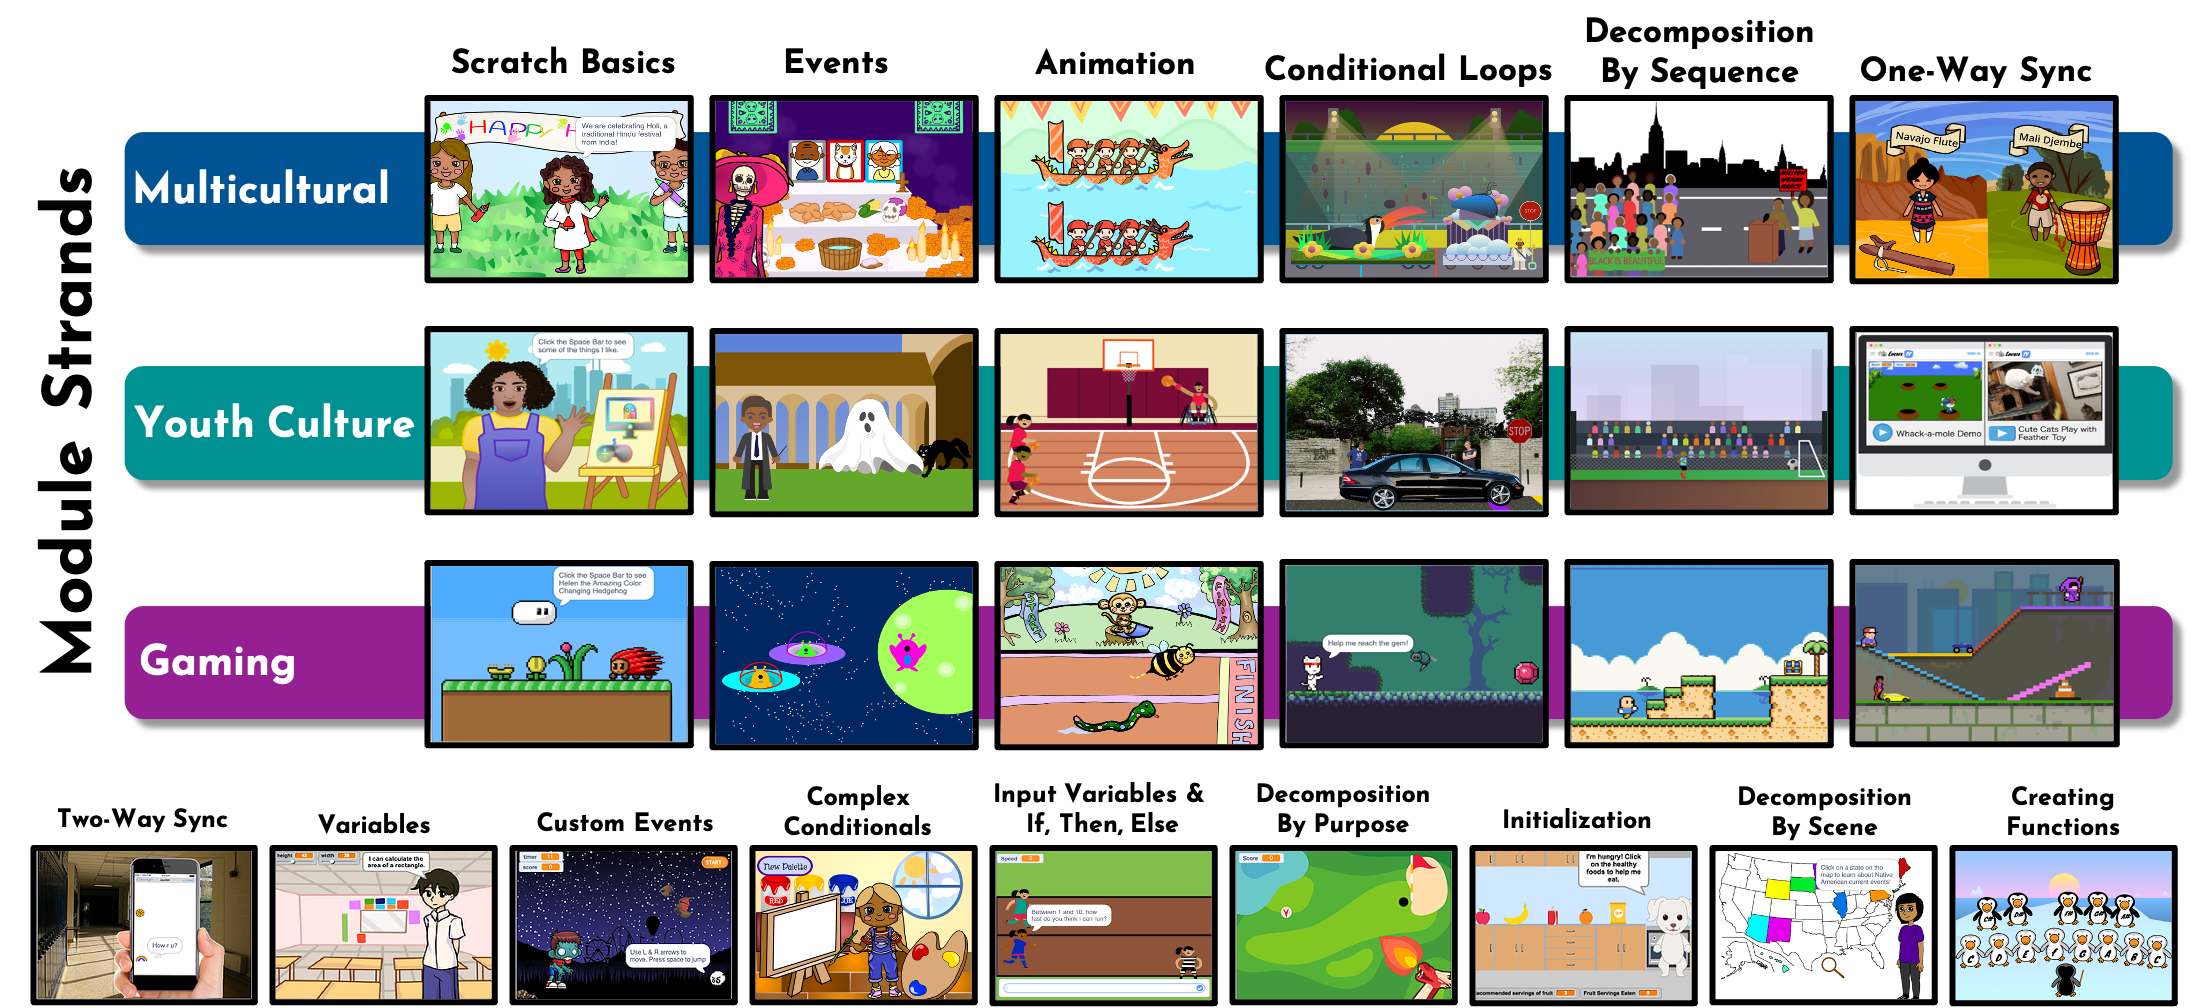
\includegraphics[width=\textwidth]{examples/EncoreStrands.png}
%     \caption{3 curricular strands, providing per-module activity choices}
%     \label{fig:my_label}
% \end{figure}

% \Scratchencore{} utilizes 2 learning and pedagogical strategies: \umc \cite{lee2011} and \ts{} \cite{salac2020tippnsee}. The \umc pedagogical strategy is used to scaffold the conceptual learning. Students first explore and modify a functioning example. Then they apply the new concept(s) to an open-ended create project\cite{authors}. %Blinded citation to UMC here.
%  %Within \Scratchencore{} this ``learn by example'' step is guided by the \ts{} learning strategy. After they have explored the project, students modify the example to try out using the CS concept they are learning. Finally, students develop an open-ended project using the CS concept focal to the module. 

% \subsection{\ts{}}
% In this section we introduce \ts{} with a focus on how \ts{} is enacted within \Scratchencore{}. \ts{} is a meta-cognitive learning strategy designed to help students learn from provided code. %\ts{} provides scaffolding for middle-school and elementary-school students to use, examine, and learn from pre-written Scratch programs. 
% \ts{} is divided into 4 question phases (``Preview'', ``Observe'', ``Predict'', and ``Explore') to help them explore the example project prior to making modifications. %``Preview'' sections instruct the students to read the introductory information about the Scratch project to contextualize the project and clarify the activity's learning goals. ``Observe'' questions involve observing an example program operation. ``Predict'' questions involve making predictions about how the code may operate. ``Explore'' questions involve observing an example program operation after making changes to the program. While these definitions categorize question type for the researchers, the students are guided through the ``Preview'', ``Observe'', ``Predict'', and ``Explore'' questions through instructions through scaffolding abbreviated to \ts{}. % Scratch is a popular programming language and development environment used in elementary-schools ~\cite{flannery2013designing} 

% TIPP stands for:
% \begin{itemize}
%     \item \textbf{T}itle: What is the title of the project? Does it tell you something about the project?
%     \item \textbf{I}nstructions: What do the instructions tell you to do?
%     \item \textbf{P}urpose: What is the purpose of this activity?
%     \item \textbf{P}lay: Run the project and see what it does! Which sprites are doing the actions?
% \end{itemize}

% \begin{figure}[h]
%     \centering
%    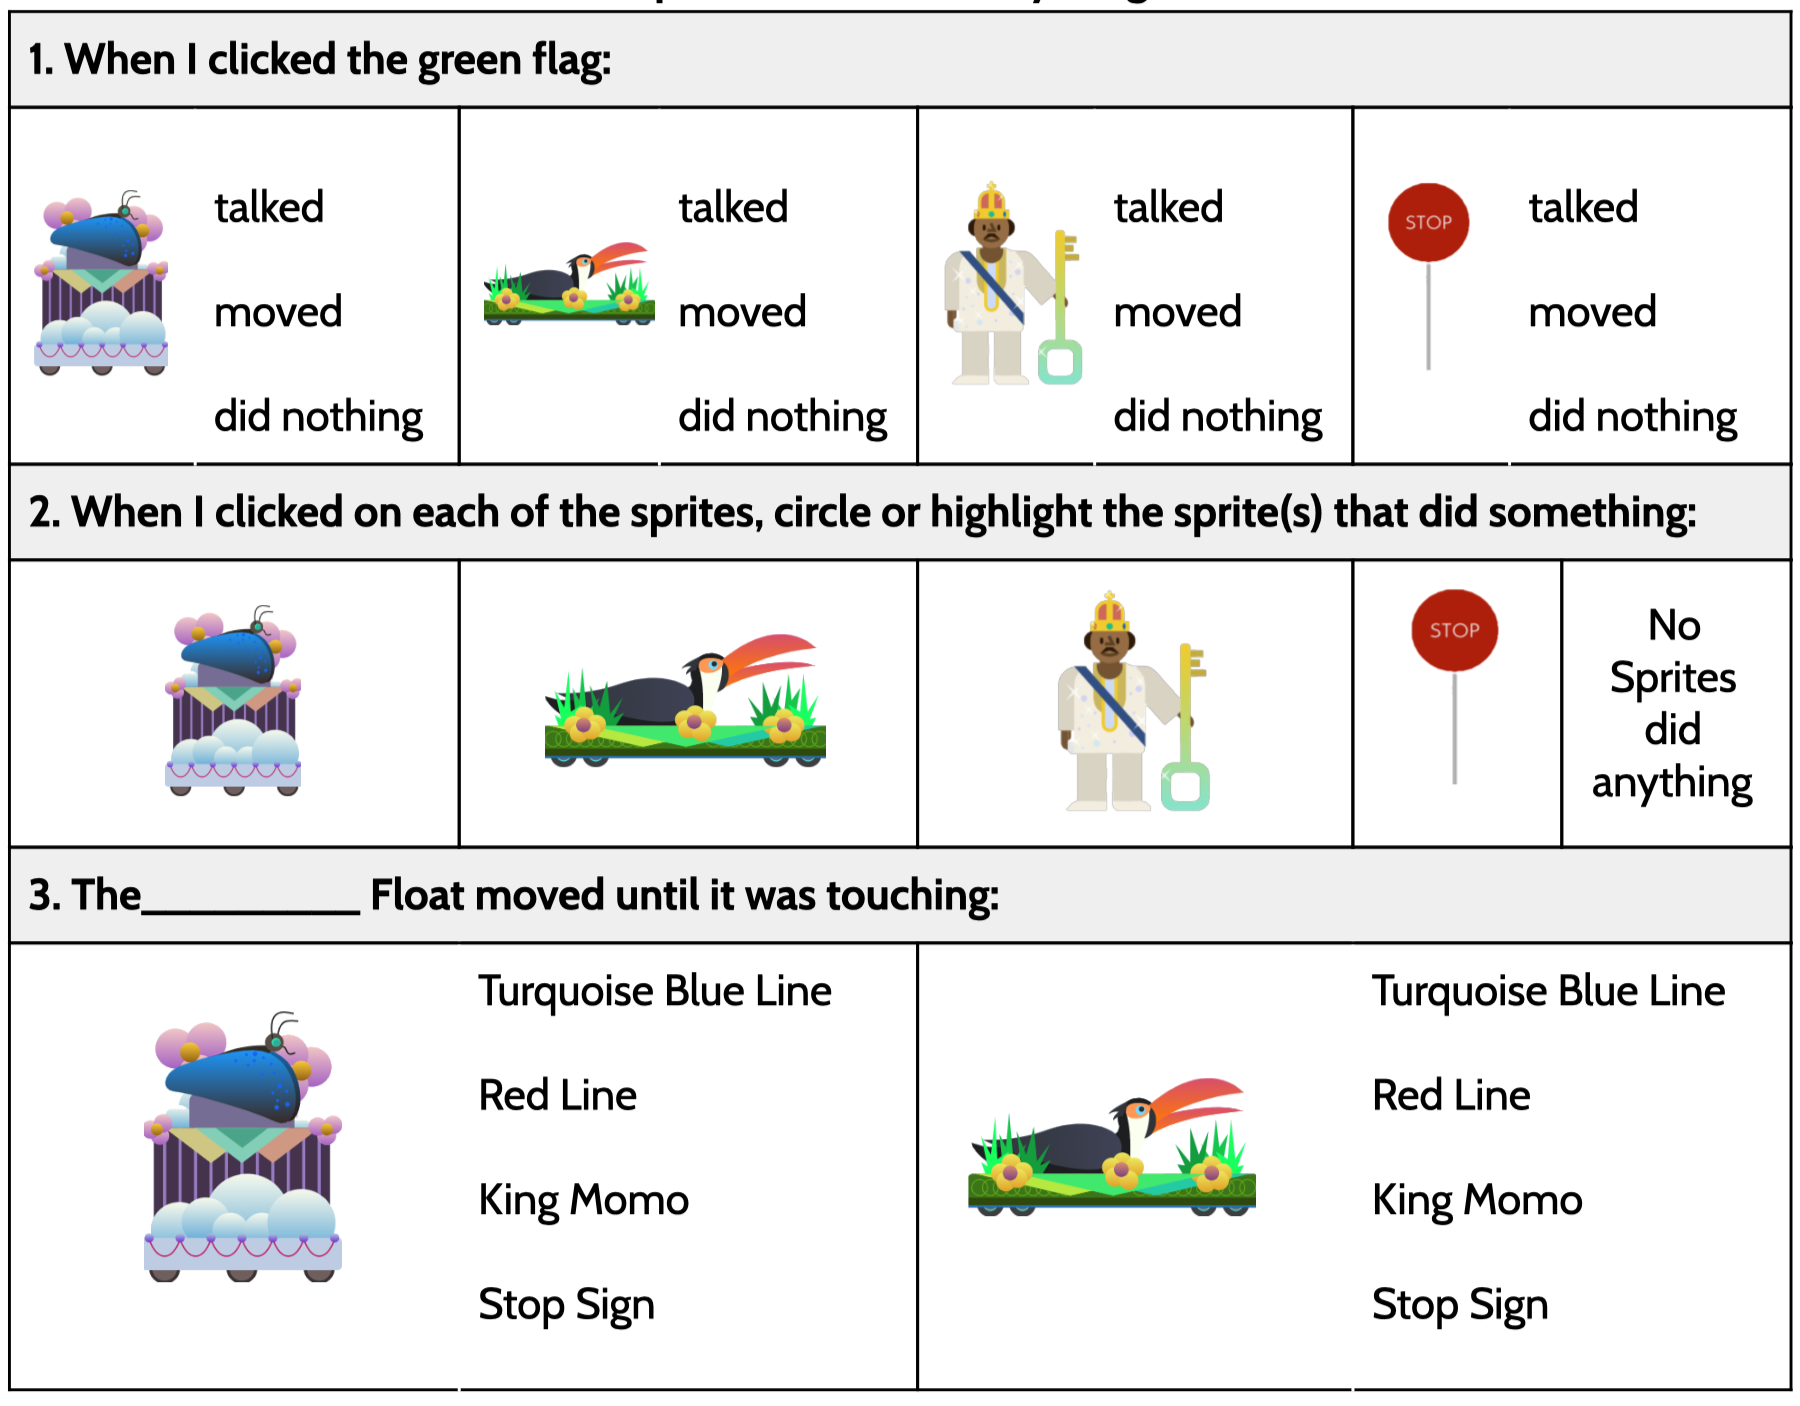
\includegraphics[width=.6\linewidth]{examples/TIPP_Example.png}
%     \caption{TIPP worksheet guides students through mindfully playing and observing the provided Scratch project.}
%    \label{fig:tipp}
% \end{figure}

% The TIPP portion of \ts{} was developed following scaffolding strategies that were effective in supporting student reading comprehension~\cite{sharonv}. Students first \textbf{Preview} the project by reading the Title, Instructions, and Purpose (TIP) of the Scratch project in order to orient the student to the both how to interact with the project and the learning goals of the activity. The students then \textbf{Observe} what the program does by Playing (P) the provided program. The questions in the accompanying worksheet are organized to ask the student to identify, for each user \textit{event}, what \textit{sprite} performed what \textit{actions} because Scratch code is organized by these 3 elements. %The first 3 steps, TIP, instruct the students to preview the project by reading the title, instructions, and purpose. They then Play the project, observing closely what happens as a result of user input. 

% Figure \ref{fig:tipp} provides an example of TIPP questions asking students about a Scratch project in \Scratchencore{} M4:CondLoops. After an initial discussion about repeated actions and how repeated actions can end after a set number of repetitions or based on a condition becoming true, students are given example code from a project with a Carnival setting reflecting the Multicultural strand. The example program includes scripts for 3 sprites: a Butterfly Float, a Toucan Float, and a king figure. A stop sign sprite is also included in the program, but it has no scripts associated with it. When the green flag is clicked, the Butterfly Float sprite moves until it touches the stop sign sprite, illustrating how a conditional loop works. The questions provided in Figure \ref{fig:tipp} focus on the final P of TIPP, Playing, by asking students to interact with the project in particular ways, such as clicking the green flag or clicking certain sprites. Students are then also tasked with noticing resulting movements or sounds from the aforementioned interaction via questions requiring them to 
% distinguish whether a given sprite talked, moved, or did nothing (question 1), note if a given sprite responded to any of the Sprites being clicked (question 2), and record when a given sprite stops moving (question 3). These questions are carefully chosen to highlight important aspects of the example code.

% \begin{figure}[h]
%     \centering
%     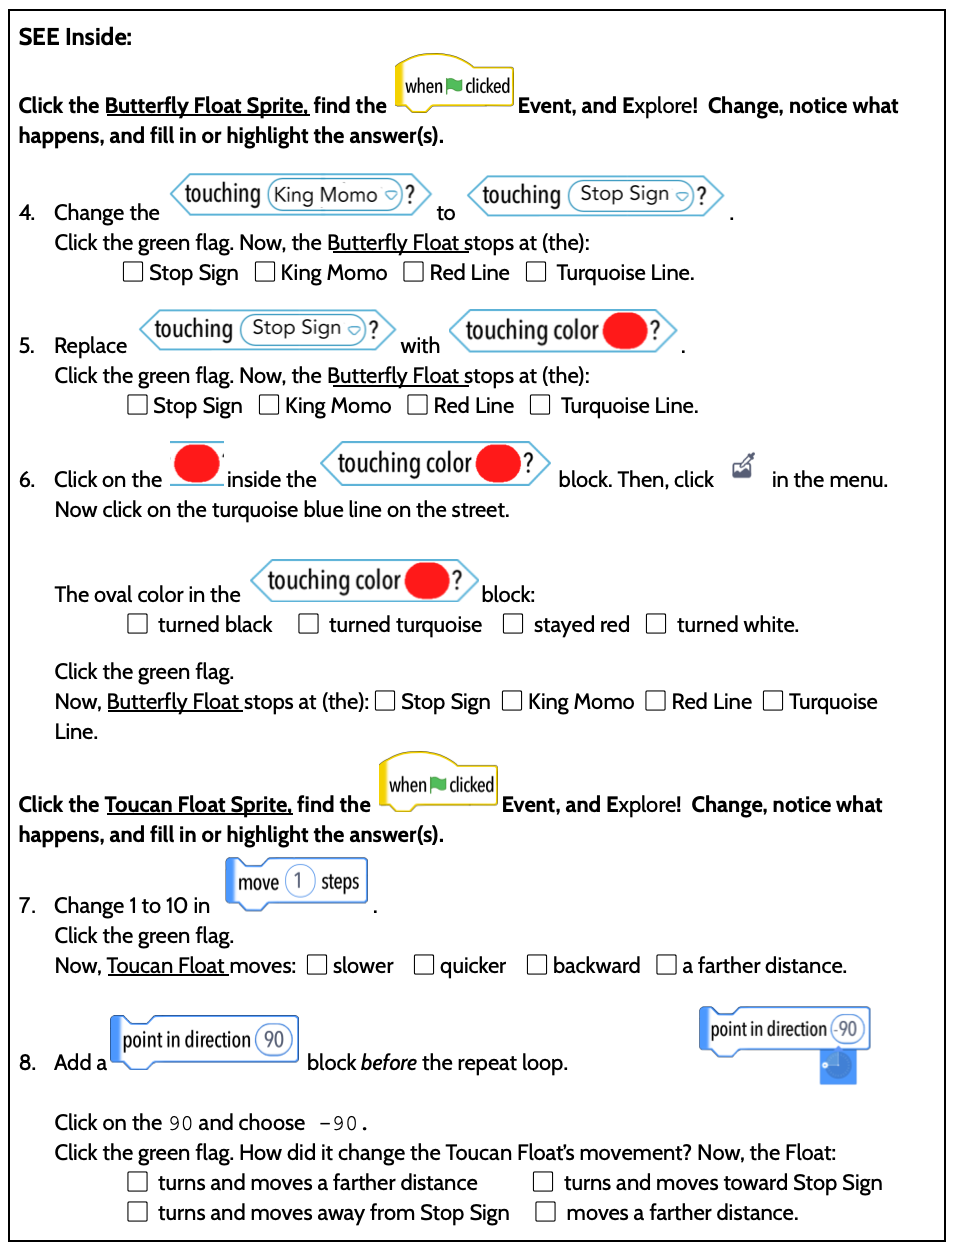
\includegraphics[width=.6\linewidth]{examples/SEE_Example.png}
%     \caption{SEE worksheet helps students navigate Scratch and learn blocks through deliberate exploration (tinkering).}
%     \label{fig:see}
% \end{figure}

% SEE stands for:
% \begin{itemize}
%     \item \textbf{S}prites: Click on the the \textbf{S}prite that you want to learn from or change.
%     \item \textbf{E}vents: Look at the \texttt{event} blocks starting the scripts.
%     \item \textbf{E}xplore: Try different changes to the scripts and observe what happens!
% \end{itemize}

% Students are then instructed to click the ``SEE INSIDE'' button on the Scratch interface and answer questions about and with the code. The SEE portion of \ts{} was inspired by the work of researchers creating reading comprehension writing structure education plans ~\cite{sdymock}. SE (sprite, event) is a navigational scaffold to help students find code in Scratch. To find code, students are instructed to click on a specific Sprite (S) and locate a specific Event (E). Students first answer a series of ``Predict'' questions asking them to inspect the code, reflect on what they observed during Play, and then predict what blocks in specific scripts caused the specific actions they observed. %, and Explore (E). %SE represents the ``Predict'' stage, in which they inspect the code and connect the code they are seeing to the actions they observe. In Scratch, code is organized by sprite and event, which inspired the name of this section of the worksheet. %In order to provide a reason to look at the code, we have them predict what blocks performed what actions (Figure ~\ref{fig:see}). Finally, they then Explore new blocks by making small changes to them, including changing the arguments, order, and number of blocks. 
% %The students are guided through the process of making predictions according to what they see in the code, predicting the role of the blocks that they ``see inside'' the program in the actions they observed in the Play phase of \ts{}. 
% Finally, the students \textbf{Explore} (E) through making changes to the code and reporting the changes in the behavior of their sprites as a result to their changes. For example, by adding, removing, or moving blocks, or changing the parameters of a specific block, and reporting how it changes the program, the students are able to gain a detailed understanding of that block and how to use it. 

% Figure \ref{fig:see} provides the SEE questions complementing the TIPP questions about Conditional Loops introduced earlier in Figure \ref{fig:tipp}. The SE navigational scaffold in this example worksheet instructs students to locate the ``when green flag clicked'' event of the Butterfly Float sprite. Then, students are guided through exploration by way of changing the fields of the \texttt{touching} block (question 4), replacing the \texttt{touching} block with a \texttt{touching color} block (question 5), and then changing the field of the \texttt{touching color} block (question 6). Students are then guided to the \texttt{when green flag clicked} event of the Toucan Float sprite via another SE scaffold and asked to change the fields of a \texttt{move} block as well as insert a new \texttt{point in direction} block.

% In this project's Modify step, students are asked to choose different float costumes, stop the floats at different locations, change the speed of the float movement, and add \texttt{say} blocks. The Create step is much more open-ended and has the students create projects based on design prompts. If students have extra time, extension activities are provided including adding other sprites, having sprites perform repeated actions until a condition becomes true, and adding sounds.

% % Past research ~\cite{salac2020tippnsee} has shown that students who used /ts had significantly stronger outcomes than students who did not. In that curriculum, the goal was for students to form an accurate mental model of a program, as expressed through Scratch. Like Sorva et al. [ Juha Sorva. ``Notional Machines and Introductory Programming Education''. In: ACM Transactions on Computing Education 13 (June 2013), 8:1–8:31. doi: 10.1145/2483710.2483713.], our definition of ``understanding'' was if students could predict the outcome of a certain script run by the computer or if students could postulate which script produced a certain outcome. Analyzed with the Block model [Carsten Schulte. ``Block Model: an educational model of program comprehen- sion as a tool for a scholarly approach to teaching''. In: Proceedings of the Fourth international Workshop on Computing Education Research. 2008, pp. 149–160.], this is a structural understanding of Scratch. In assessments designed for students to demonstrate their understanding, /ts students outperformed control students in questions of moderate to advanced difficulty. Figure 5 shows performance on questions related to loops, and student scores are normalized to the treatment group. Asterisks indicate a statistically-significant difference in performance between the 2 groups. Our goal in this study is to investigate behavioral differences in \umc artifacts and /ts worksheets that may have led to such dramatic performance differences.

% %Examples of useful RCS which were incorporated into the design of \ts{} include Previewing and Text Structures \cite{tippnsee}. \pratham{todo - Previewing and Text Structures general descriptions}

% %\ts{} in particular combines many facets of the aforementioned MLS to scaffold ... \pratham{how Previewing and Text Structures can be used in \ts{}, as described in \ts{} analysis} \ts{} is expanded on in the next section.

\section{Methods}
\label{sec:methods}
To quantify the extent to which the \cvd{} pandemic and subsequent disruptions to in
person learning affected the efficacy of and extent to which CS instruction took place at the elementary and middle school level we collected both large scale as well as individualized data of \Scratchencore{}.

\subsection{Data Collection}
We collected both large scale, publicly available, data as well as individualized student data from
classes in our partner district. The first portion of our data consists the metadata for every
 single project that was `remixed' from the Scratch Encore account and then shared publicly.
 A total of 26,826 projects were found by our web scraper of which 26,009 were created
 between August 2018 and July 2021. We also looked at teacher registrations for the 
 \Scratchencore{} curriculum; these include basic demographic information such as email
 addresses, teaching position, type of students, and location. The individualized school data
 was reported by teachers from our partner district and include the number of \Scratchencore{}
 modules completed each year as well as the completed Scratch projects for each of their
 students. All teachers taught the \Scratchencore{} for at least 2 out of the last 3 years: either
 before and during the pandemic year or during the pandemic year and in the subsequent
 online only year.

\subsection{Data Analysis}

Our large scale analysis focused mainly on \Scratchencore{} activity over time. For the
student remixes we had enough data where we could sort the projects by their creation
time-stamps and get a meaningful picture of how much instruction was taking place on
any given day over the past three years. For teacher registrations we first filtered out entries
from people requesting access who indicated that they were not teachers (this was a relatively small number
and consisted mainly of researchers) and also kept track of teachers who belonged to
our partner district by checking the email addresses used during registration. We then sorted the registrations based on their timestamps
to see how many teachers were requesting access on any given month.\\
  For the teacher data, we had teachers from our partner district submit anonymized copies
of  their student's completed worksheets as well as a list of all the student's scratch projects.
From this we were able to determine how many modules of the \Scratchencore{} each
teacher had completed that year. We additionally ran all of the student's scratch projects 
through an automated assessment tool which parses the code to analyze the extent to which
they project satisfies the required tasks. For example, if a project requires a student to
make a animate sprite movement, the autograder would parse the code and search for
``move'' and ``wait'' blocks nested within a “repeat” block. Given the open-ended nature
of coding it is possible for students to create a project that satisfies ``the spirit'' of the
requirements but does so in a way that is so unique or convoluted that it would be missed 
by the autogrades, nevertheless, these situations are extremely rare.
% Our analysis focused on 3 sources of data: \ts{} worksheets, computational artifacts (Modify and Create projects), and student demographic surveys. The analysis primarily focused on the \ts{} worksheets, with data from computational artifacts and demographic surveys being used to situate emerging findings and gain an understanding of additional factors that might be driving behavior found in worksheet data.

% To further contextualize and understand trends observed in the data, all worksheet questions were analyzed in 3 distinct ways. First, each question was categorized based on what students were asked to do and how it aligned to the \ts{} phase, either ``Observe'', ``Predict'', or ``Explore'', described above. %``Observe'' questions ask the students to observe and report what they see happens when they run the code or when they look inside the code at the scripts. ``Predict'' questions ask the students to predict the function of a block without changing the code, requiring students to demonstrate a theoretical understanding of the function of blocks. ``Explore'' questions ask the students to retrospectively determine the function of a block after changing the code and observing the results. 
% Questions were well-defined in one of these categories during the creation of the worksheets and did not require sorting by researchers. Questions that did not fall into any of the categories (such as asking students to report the number of costumes in order to encourage students to discover the costumes tab) were removed from analysis.

% The second phase of analysis involved researchers splitting questions into correct and either blank or incorrect answers and extracting trends or patterns. This led to the second round of analysis, focusing on question position and the relationship between the language / concept in the block and usage in everyday life.

% Analysis on where the question was positioned within the worksheet structure was straightforward. This was an objective categorization, with 9 questions per worksheet (3 per section) being labelled as ``first'', ``middle'', or ``last'' within the ``Observe'', ``Predict'', and ``Explore'' sections as described in the previous paragraph. 

% A more complex analysis investigated the relationship between the language used on the block and related everyday meaning of those same terms. For example, some questions asked students to predict which block made a sprite move, and the answer was the \texttt{move} block, showing a direct mapping between programmatic meaning and everyday meaning. On the other hand, if a sprite were to rotate, in everyday language, this would still be considered a \texttt{move}, but it would not involve the \texttt{move} block in Scratch, so this would be a mismatch between Scratch word usage and everyday usage. We then developed a coding scheme to classify this relationship: ``Everyday True Positive'', ``Everyday False Positive'', and ``X-Y Coordinate''. ``Everyday True Positive'' involved questions concerning blocks or concepts that had an everyday, real-world interpretation that matched with their function in Scratch (e.g. the first example of move). For example, the multiple choice question, ``Which block makes Neha talk?'' requires the answer, ``say (Hi, I'm Neha) for (2) seconds''.  ``Everyday False Positive'' involved questions concerning blocks or concepts that had an everyday, real-world interpretation that did not match with their function in Scratch (e.g. the example of move and rotate). Finally, a third group was identified, which involved school-based knowledge that did not have an everyday understanding. After analysis, it was determined that this category all pertained to questions on the x-y coordinate system, so we renamed it to ``X-Y Coordinate'' for clarity. For example, the \texttt{go to X: () Y: ()} block sets the sprite's X and Y position to the provided number, moving the sprite on the screen without animation, causing the sprite to jump to the spot corresponding with the new providing position. Questions that ask students to change a value in a \texttt{go to X: () Y: ()} block and determine if the sprite has moved closer to another sprite or further from another sprite would require the student to have and apply elementary or middle-school learned knowledge of the Cartesian coordinate plane to be able to accurately guess the result, and thus, were placed in the ``X-Y Coordinate'' category. 

% %However, questions that ask the students to predict which block makes a sprite start in the same place with the answer being \texttt{go to X: () Y: ()}, were labeled as ``Everyday True Positive'' because the ``go to'' is likely to be intuitive to a learner and does not require knowledge of the Cartesian coordinate plane.

% The first round of coding split ``Predict'' and ``Explore'' questions (55 questions total) into just 2 categories: ``Everyday'' versus ``School'' (where ``School'' was anything that did not meet the everday definition and contains both ``X-Y Coordinate'' and ``Everyday False Positive''). 3 researchers made 2 cycles of developing and modifying category definitions, followed by independent coding of the questions and a discussion to resolve any disagreements. After refining the definitions further and re-coding the data, we reached a 45.50\% agreement (Fleiss' \begin{math}\kappa\end{math} = 0.265). The low agreement and IRR is due to the small dataset. Therefore, all data was triple coded, and any outstanding disagreements were resolved through discussion to 100.00\% agreement. We then divided the ``School'' questions into ``X-Y Coordinate'' or ''Everyday False Positive''. Due to the small set of questions, researchers coded the categories together and did not calculate agreement.
% %We were inspired to create these categories by a pattern noticed while coding student correctness data. We decided to attempt to understand how language and previous knowledge (in terms of whether it was acquired from school or everyday common sense) affects students’ performance on /ts questions. 

% %The categories that this inspired are as follows. ``Everyday True Positive'' questions are questions concerning blocks or concepts that a have a real world, everyday interpretation that matches with their role in Scratch. For example, the \texttt{move () steps} block is an ``Everyday True Positive'' block as it moves the sprite forward in the direction it is already facing for the provided number of steps. ``Everyday False Positive'' questions are questions concerning blocks or concepts that a have a real world, everyday interpretation that does not match with their role in Scratch. 

% %not sure if we want to include pictures of these examples too but just in case I uploaded them to the images for this doc. they're called school example.png, tpexample1.png, tpexample2.png



% Completion and accuracy rates of the worksheets were then examined against each of these 3 sets of categorizations to observe whether there was a relationship between student performance on questions and their characteristics. To see if there was any association between student responses and the type of question (``Observe''/``Predict''/``Explore''), type of knowledge (``Everyday'' compared to ``X-Y Coordinate'' knowledge) and question position, the chi-square test of independence was used. We report \begin{math}\chi\end{math} and \begin{math}p\end{math} values from this test, with \begin{math}p<.05\end{math} as our threshold for significance. In addition to characteristics of the questions themselves, we also examined factors related to students and their environment through the demographic survey responses. Specifically, we examined whether students' performance on questions varied depending on whether their parent reported that they had previous programming experience or previously struggled with mathematics homework, both of which were represented as binary ``yes'' or ``no'' variables. To compare performance across programming experience, the non-parametric Kruskal-Wallis test was used as some categories of parent-reported programming experience, such as having both school and informal experiences, had very small numbers of students and violated parametric assumptions. We report \begin{math}\chi\end{math} and \begin{math}p\end{math} values for statistical significance and the \begin{math}\eta^2\end{math} value for effect size. To compare across parent-reported math difficulty, we used the parametric Anova F-test for Modules 1 and 2, which more students completed and whose distribution met the assumptions of the F-test. Its nonparametric analog, the Kruskal-Wallis test, was used for Modules 3 and 4, because of small sample size. We report \begin{math}F\end{math}, \begin{math}p\end{math}, and \begin{math}\eta^2\end{math} values from the Anova F-test. We also explored whether a particular teacher or classroom affected student performance, using the Kruskal-Wallis test because of some small class sizes. Finally, Modify and Create project completion rates were compared to \ts{} worksheet completion rates to assess the degree to which \ts{} encourages creativity and deepens understanding of CT concepts in middle-grade students.

% %Data was analyzed to better understand 2 aspects of student work: completion of technical elements and variations from the structured tasks.

% %For completion of technical elements, the Scratch programs from classrooms were analyzed using static analysis to determine if the work met project requirements and if any module extensions were attempted. This data was then used to calculate a completion percentage for each student. This percentage represents the total number of module requirements completed by students for each activity they attempted in Modules 1-4. %We then analyzed these results to identify teacher or grade level patterns in terms of program completion. Students attempted between 1 and 8 activities. 

% %Since some teachers within our data set taught students in multiple classes, we first analyzed intraclass correlation (ICC) for a hierarchical model predicting completion score by teacher and grade. Due to the low ICC (ICC=0.03), it was determined that a hierarchical model was not necessary and general linear regression models were used to analyze correlations between teacher, grade, and student completion. A multiple regression model was run to determine the influence of teacher and grade on completion percentage and 2 simple linear regressions were run to separately determine the influence of each variable (teacher and grade) on completion percentage. Assumptions of normality, linearity, homoscedasticity and independence with each regression model were examined through statistical testing and analysis of graphs. All assumptions were determined to be met. Analysis of Variance (ANOVA) were used to compare across the 3 models. 

% %To understand decisions students made in the Create projects, a number of analyses were conducted. First, we analyzed the blocks used and categorized them based on when they were introduced to students (in a previous module, the current module, or a future module). Next, Scratch projects from a subset of students were inspected to understand in what ways students completed tasks beyond the requirements of the project. Researchers performed qualitative analysis, recording project characteristics such as the number of sprites, backdrops, and costumes used and how students changed their final projects as compared to the starter project that most students were given for the create tasks. These data were then analyzed for frequency. Finally, static analysis modules were coded in JavaScript to analyze the Scratch code in all student projects in a studio and produce a spreadsheet of results. These looked for not only the required elements, but also examples of the types of additional actions that had been identified through hand inspection. 

% %Finally, when differences were identified between teachers, observation notes were inspected to discover any differences in how teachers ran their classrooms. 

% % Scratch LEGO pictures

% In order to find out whether worksheet performance correlated with project completion, the programs written in all of the Modify and Create projects were analyzed using static analysis to determine completion rates for a set of predetermined requirements and extension prompts, which were provided on students' project planning worksheets. Examples of these requirements include adding a script for a given sprite, modifying a \texttt{say} block for at least 1 sprite, and modifying at least 1 sprite's costume. To extract data from \ts{} worksheets and demographic surveys, which were originally completed by hand, answers were manually transcribed into spreadsheets and checked by multiple researchers. Worksheet answers were then analyzed for completion and accuracy. %Questions where the correct answer was to leave the question blank were omitted from the analysis, as an attempt to determine whether the student intentionally left it blank could not be made. 

\newcounter{findingnum}

\section{Results}

We first compare the \Scratchencore{} project activity levels as well as teacher registrations
during the pre-pandemic, pandemic,
and online school years in order to determine the extent to which the \cvd pandemic affected
CS instruction. Then we take a look at data from our partner district to determine the extent
to which the pandemic affected the amount of content teachers were able to cover. Finally,
we dive into individual student project completion data.



\begin{figure}
     \centering
     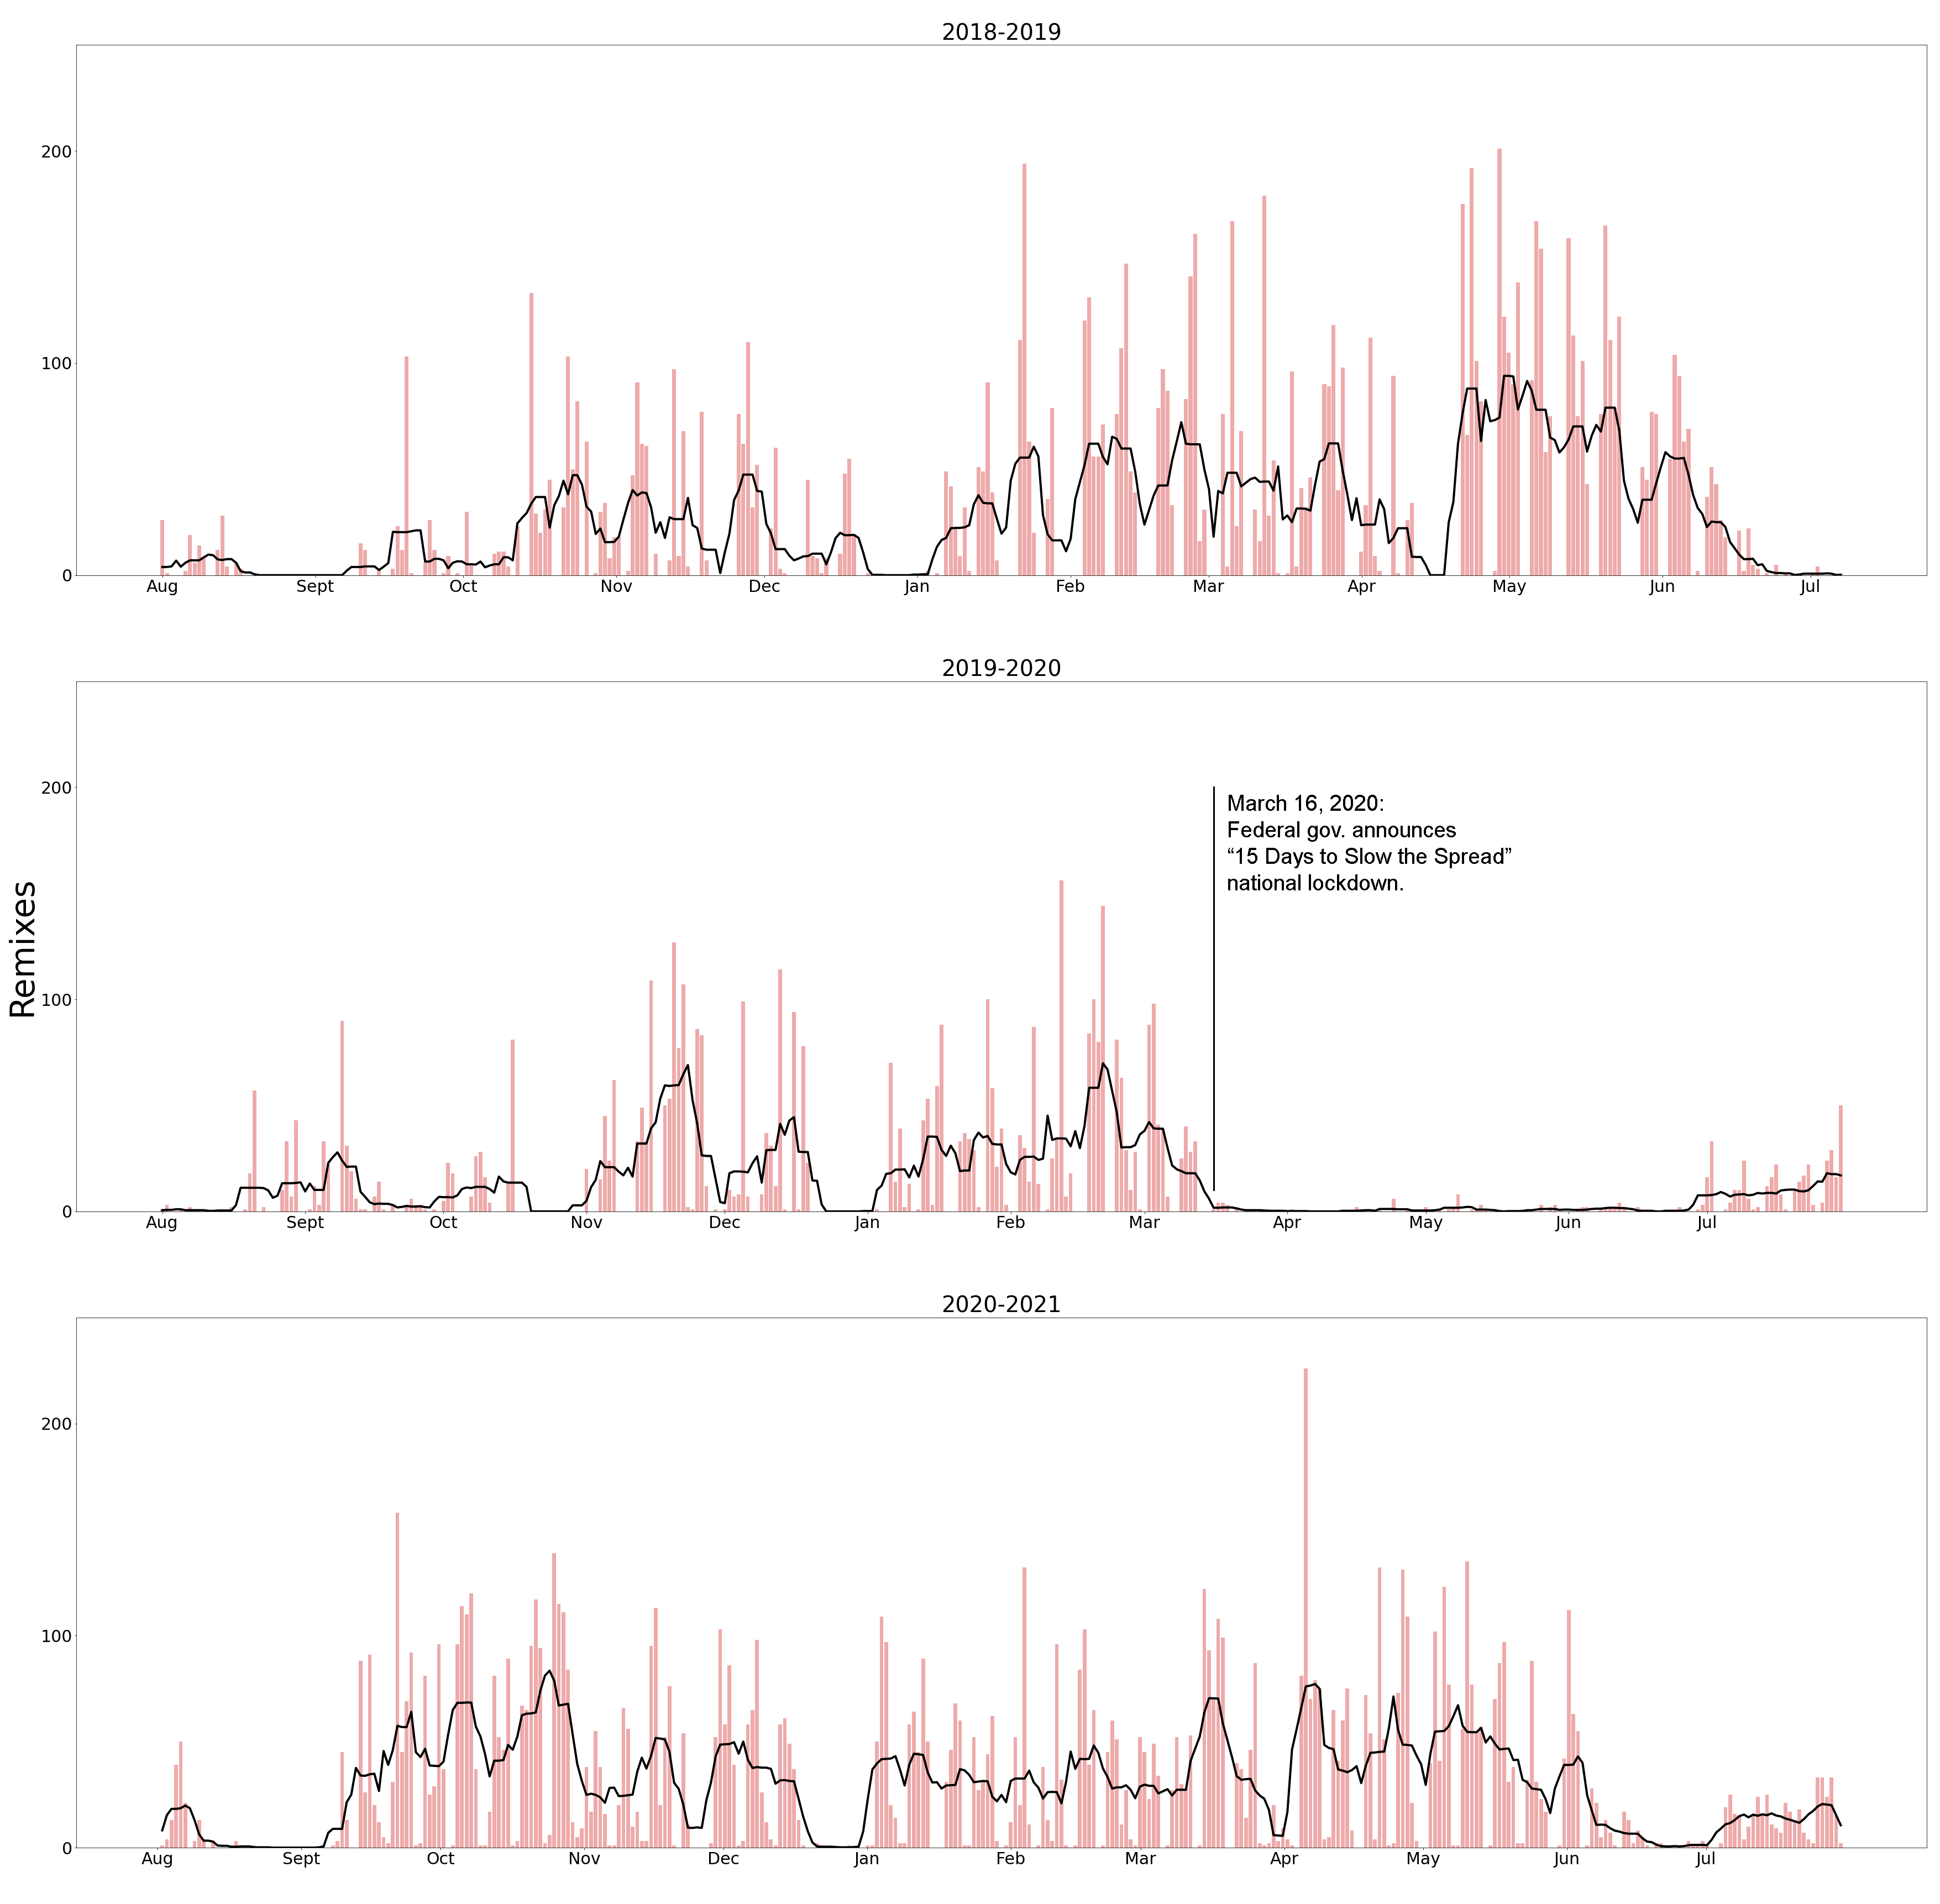
\includegraphics[width=\textwidth]{images/graphs/DailyRemixesFinal.png}
     \caption{Daily \Scratchencore{} Project Remixes for pre-pandemic, pandemic, and online school years.}
     \label{fig:daily_remixes}
    % \begin{subfigure}[t]{0.49\textwidth}
    %     \raisebox{-\height}{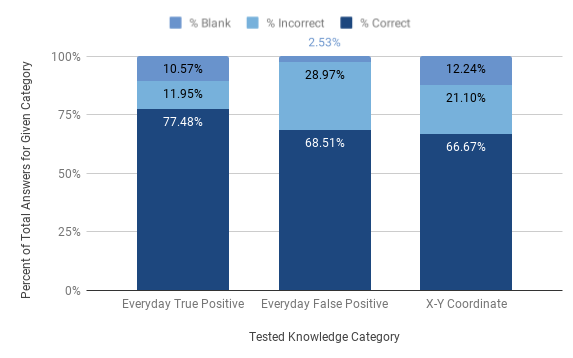
\includegraphics[width=\textwidth]{graphs/Observe_Predict_Explore_Overall.png}}
    %     \caption{Student Performance by Question Type}
    %     \label{fig:observe_predict_explore}
    % \end{subfigure}
    %     \hfill
    %     \begin{subfigure}[t]{0.49\textwidth}
    % \label{fig:curriculum_factors}
    %     \raisebox{-\height}{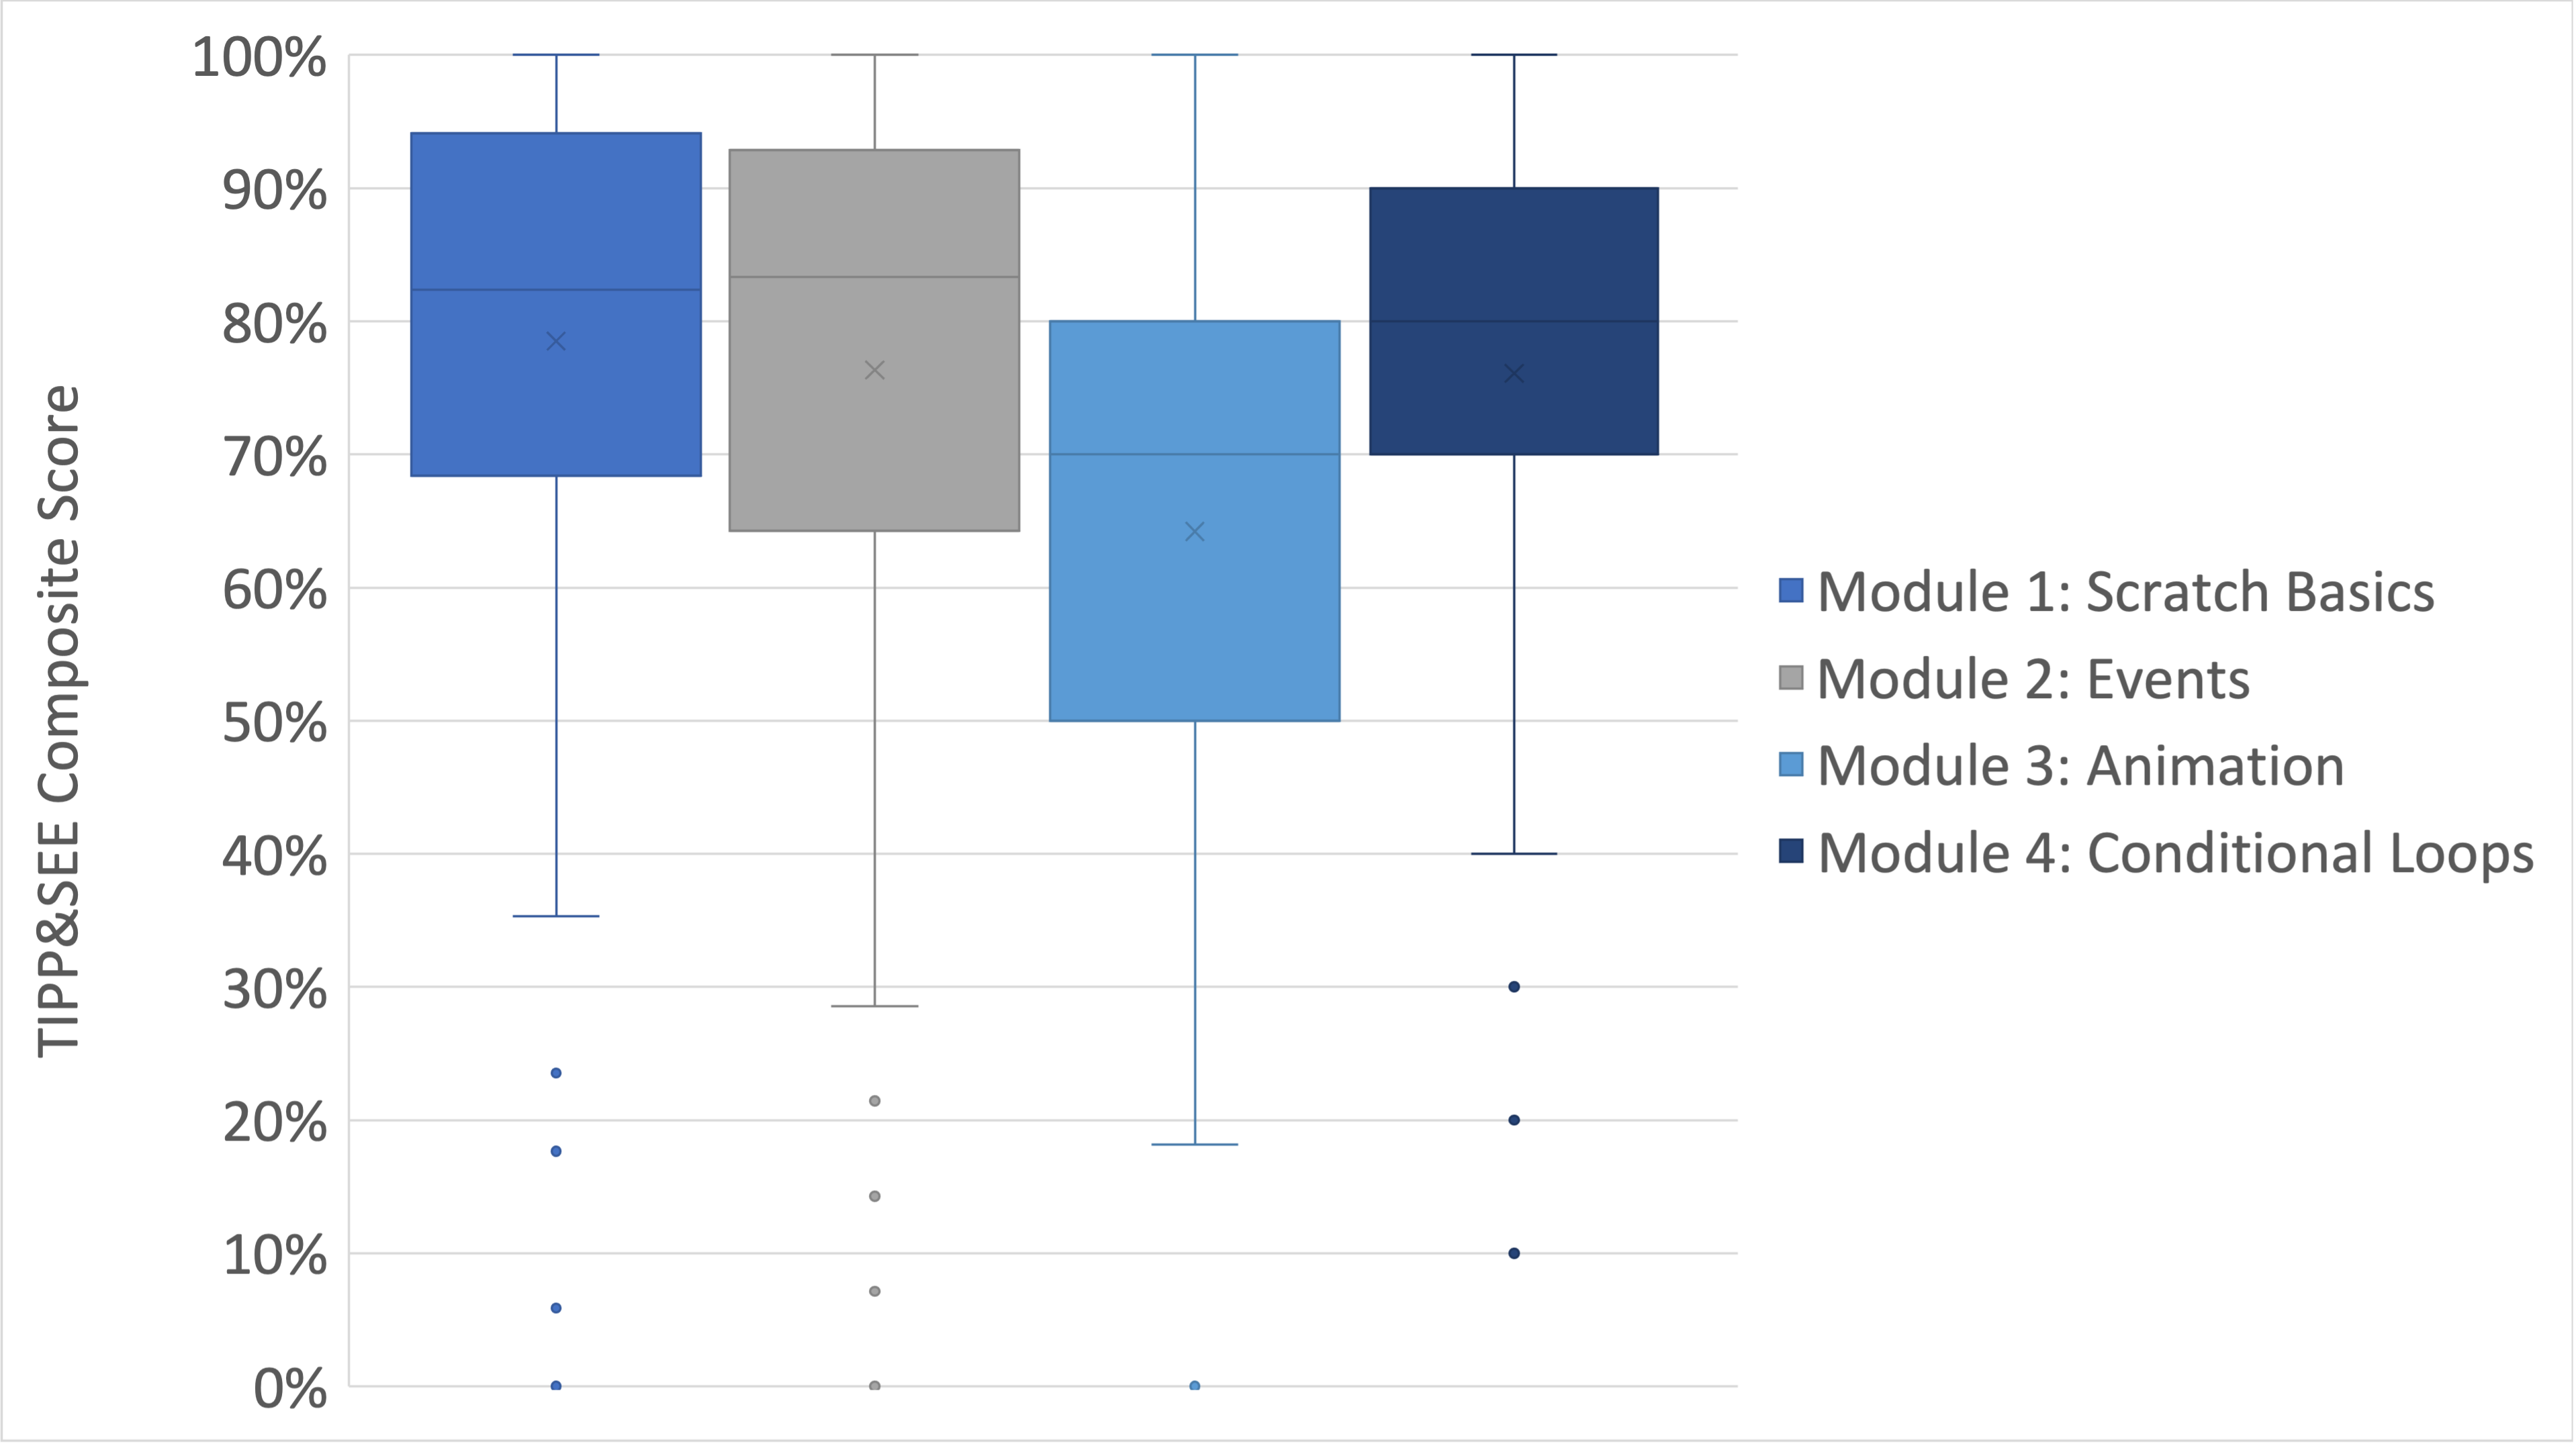
\includegraphics[width=\textwidth]{graphs/Module.png}}
    %     \caption{\ts{} Scores Compared Across \Scratchencore{} Modules}
    %     \label{fig:permodule}
    % \end{subfigure}
    % \caption{\ts{} Overall Student Performance Results}
    
\end{figure}
\subsection{Daily \Scratchencore{} Activity Over Time}
We begin by presenting the \Scratchencore{} project activity levels. Figure \ref{fig:daily_remixes}
 represents every Scratch project that was remixed from the Scratch Encore account and 
 then publicly shared from 2018 to 2021. The red bars represent the number of daily remixes 
 while the black lines represent a seven day rolling average (a format that most of us are, 
 unfortunately, intimately familiar with in a post-COVID world). Over 25,000 individual 
 projects were counted which allows us to present an extremely granular view of the extent 
 to which instruction was taking place on any given day: weekends, holidays and even 
 testing periods can be inferred from the activity taking place.\\
This level of detail allows us to present a picture of just how suddenly students and teachers
 had to transition from conventional schooling to emergency learning; the plot for the 
 2019-2020 school year shows an almost identical pattern of activity all the way through 
 March then, as most readers are bound to remember, almost overnight their world was 
 turned upside down. There is no gradual slowdown in the activity which would suggest 
 educators had been provided with the opportunity to plan an orderly transition or perhaps 
 that different districts were shutting down at different times.


\stepcounter{findingnum}
\textit{Finding \arabic{findingnum}: Instruction everywhere stopped immediately following the federal government’s declaration of a national lockdown.}
Furthermore, we see no evidence that any substantial level of instruction was accomplished
following the transition to emergency learning. By contrast, instruction levels rebounded
strongly during the post pandemic year with the first quarter of the 2020-2021 
school year showing noticeably greater activity levels than during either of the preceding 
years. The level of instruction then remains steady for the remainder of the year with less dramatic 
peaks and valleys than in the pre-pandemic year.



\stepcounter{findingnum}
\textit{Finding \arabic{findingnum}: Students attempted the most ``Observe'' questions, followed by ``Explore'' questions, and the least ``Predict'' questions.}

There is a statistically-significant association between answer type (if the student answered the question correctly, incorrectly, or not at all) and question type (\begin{math}\chi=143.7, p=2.2\times10^{-6}.01\end{math}). Across modules, students attempted questions within each section of the worksheet at different rates. Students attempted a larger percentage of ``Observe'' questions (which asked students to observe and report what they see happens when they run the code) and ``Explore'' questions (which asked students to make small modifications to existing code and tell what happens) than when they were asked to hypothesize about the function of a block (``Predict''). 

\stepcounter{findingnum}
\textit{Finding \arabic{findingnum}: Students correctly answered ``Observe'' questions at a higher rate compared to ``Predict'' and ``Explore'' questions.} 

As shown in Figure \ref{fig:observe_predict_explore}, students answered ``Predict'' and ``Explore'' questions with comparable correctness (73.47\% and 73.61\% respectively), while answering ``Observe'' questions correctly at a higher rate (79.67\%). ``Explore'' questions had the highest rate of incorrect responses (18.68\%) compared to 15.73\% incorrect for ``Predict'' questions and and 17.67\% incorrect for ``Observe'' questions. The ``Observe'' questions may have been answered more correctly because students need only view the program to answer them, whereas the ``Predict'' questions asks students to link behaviors with blocks and the ``Explore'' questions require students to make changes to the code before answering the questions.


\stepcounter{findingnum}
\textit{Finding \arabic{findingnum}: Performance varied across all modules.}
Figure \ref{fig:permodule} shows the performance in each module. While performance was strong in 3 modules, students achieved only 64\% accuracy, on average, for M3:animation. statistical analysis revealed that student worksheet correctness differed across the modules (\begin{math}F(3,668)=12.94, p=3.18\times10^{-8}, \eta^2=.0549\end{math}). Post-hoc analysis indicated that correctness was statistically-significantly different between M3:Animation and M1:Basics (\begin{math}p=1\times10^{-7}\end{math}), M2:Events (\begin{math}p=4.7\times10^{-6}\end{math}), and M4:CondLoops (\begin{math}p=6.12\times10^{-4}\end{math}). This indicates that the technique works overall, but revision may be necessary on that module.

\stepcounter{findingnum}
\textit{Finding \arabic{findingnum}: There was little correlation between \ts{} worksheet score and project score.}

Figures \ref{fig:avg_modify} and \ref{fig:avg_create} display the correlation between the average of students' scores in \ts{} and the average of students' scores in their Modify and Create projects, respectively. The correlation is low for both the Modify ($R^2$ = 0.012) and Create ($R^2$ = 0.042) projects. %The correlation between the Modify project and \ts{} score was slightly higher, potentially because this project in the Modify activity is the same project as students are introduced to through the \ts{} worksheet.%
This result shows there to be little connection between performance on the \ts{}  worksheets and performance on the projects. As we will discuss in Section~\ref{sec:compare}, this aligns with a different study on 4th-grade students.

\begin{figure}
     \centering
     \begin{subfigure}{0.49\textwidth}
        \raisebox{-\height}{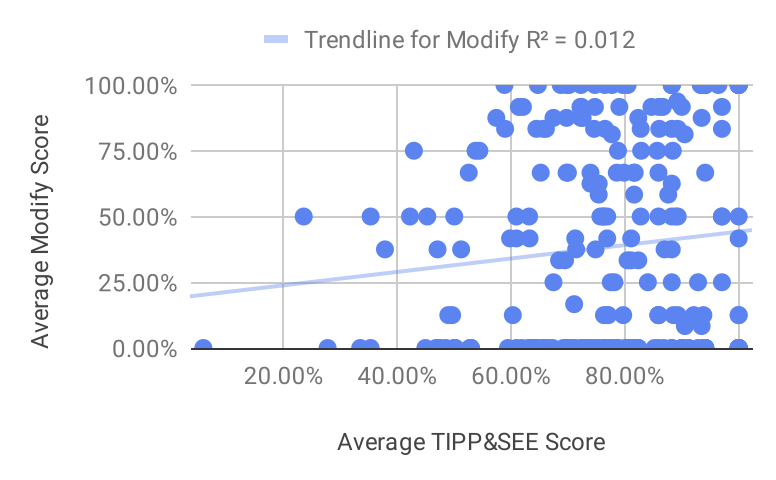
\includegraphics[width=\textwidth]{graphs/Average Modify vs. TIPP&SEE.png}}
        \caption{Average Modify scores vs. Average \ts{} scores}
        \label{fig:avg_modify}
    \end{subfigure}
    \begin{subfigure}{0.49\textwidth}
        \raisebox{-\height}{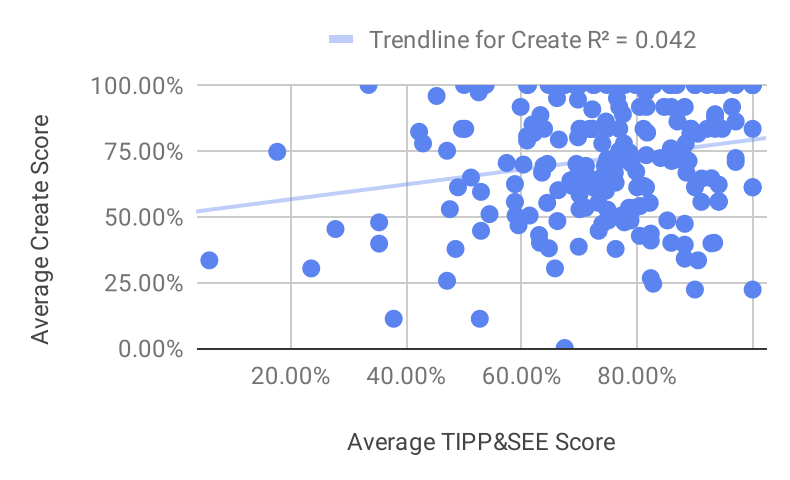
\includegraphics[width=\textwidth]{graphs/Average Create vs. TIPP&SEE.png}}
        \caption{Average Create scores vs. Average \ts{} scores}
        \label{fig:avg_create}
    \end{subfigure}
    
    \caption{Average Modify and Create scores vs. Average \ts{} worksheet scores}
\end{figure}


\subsection{Potential Performance Influences}
While overall performance was good, aggregate performance only tells us how students performed on average and could potentially hide evidence of inequity. That is, an equitable outcome would involve the consistency in performance across students based on a variety of factors. In this section, we explore many different factors that could influence performance.

\subsubsection{Classroom-Related Factors} 
We begin with classroom factors that all students in a classroom share: grade level and teacher.


\begin{figure}
     \centering
    \begin{subfigure}[t]{0.49\textwidth}
        \raisebox{-\height}{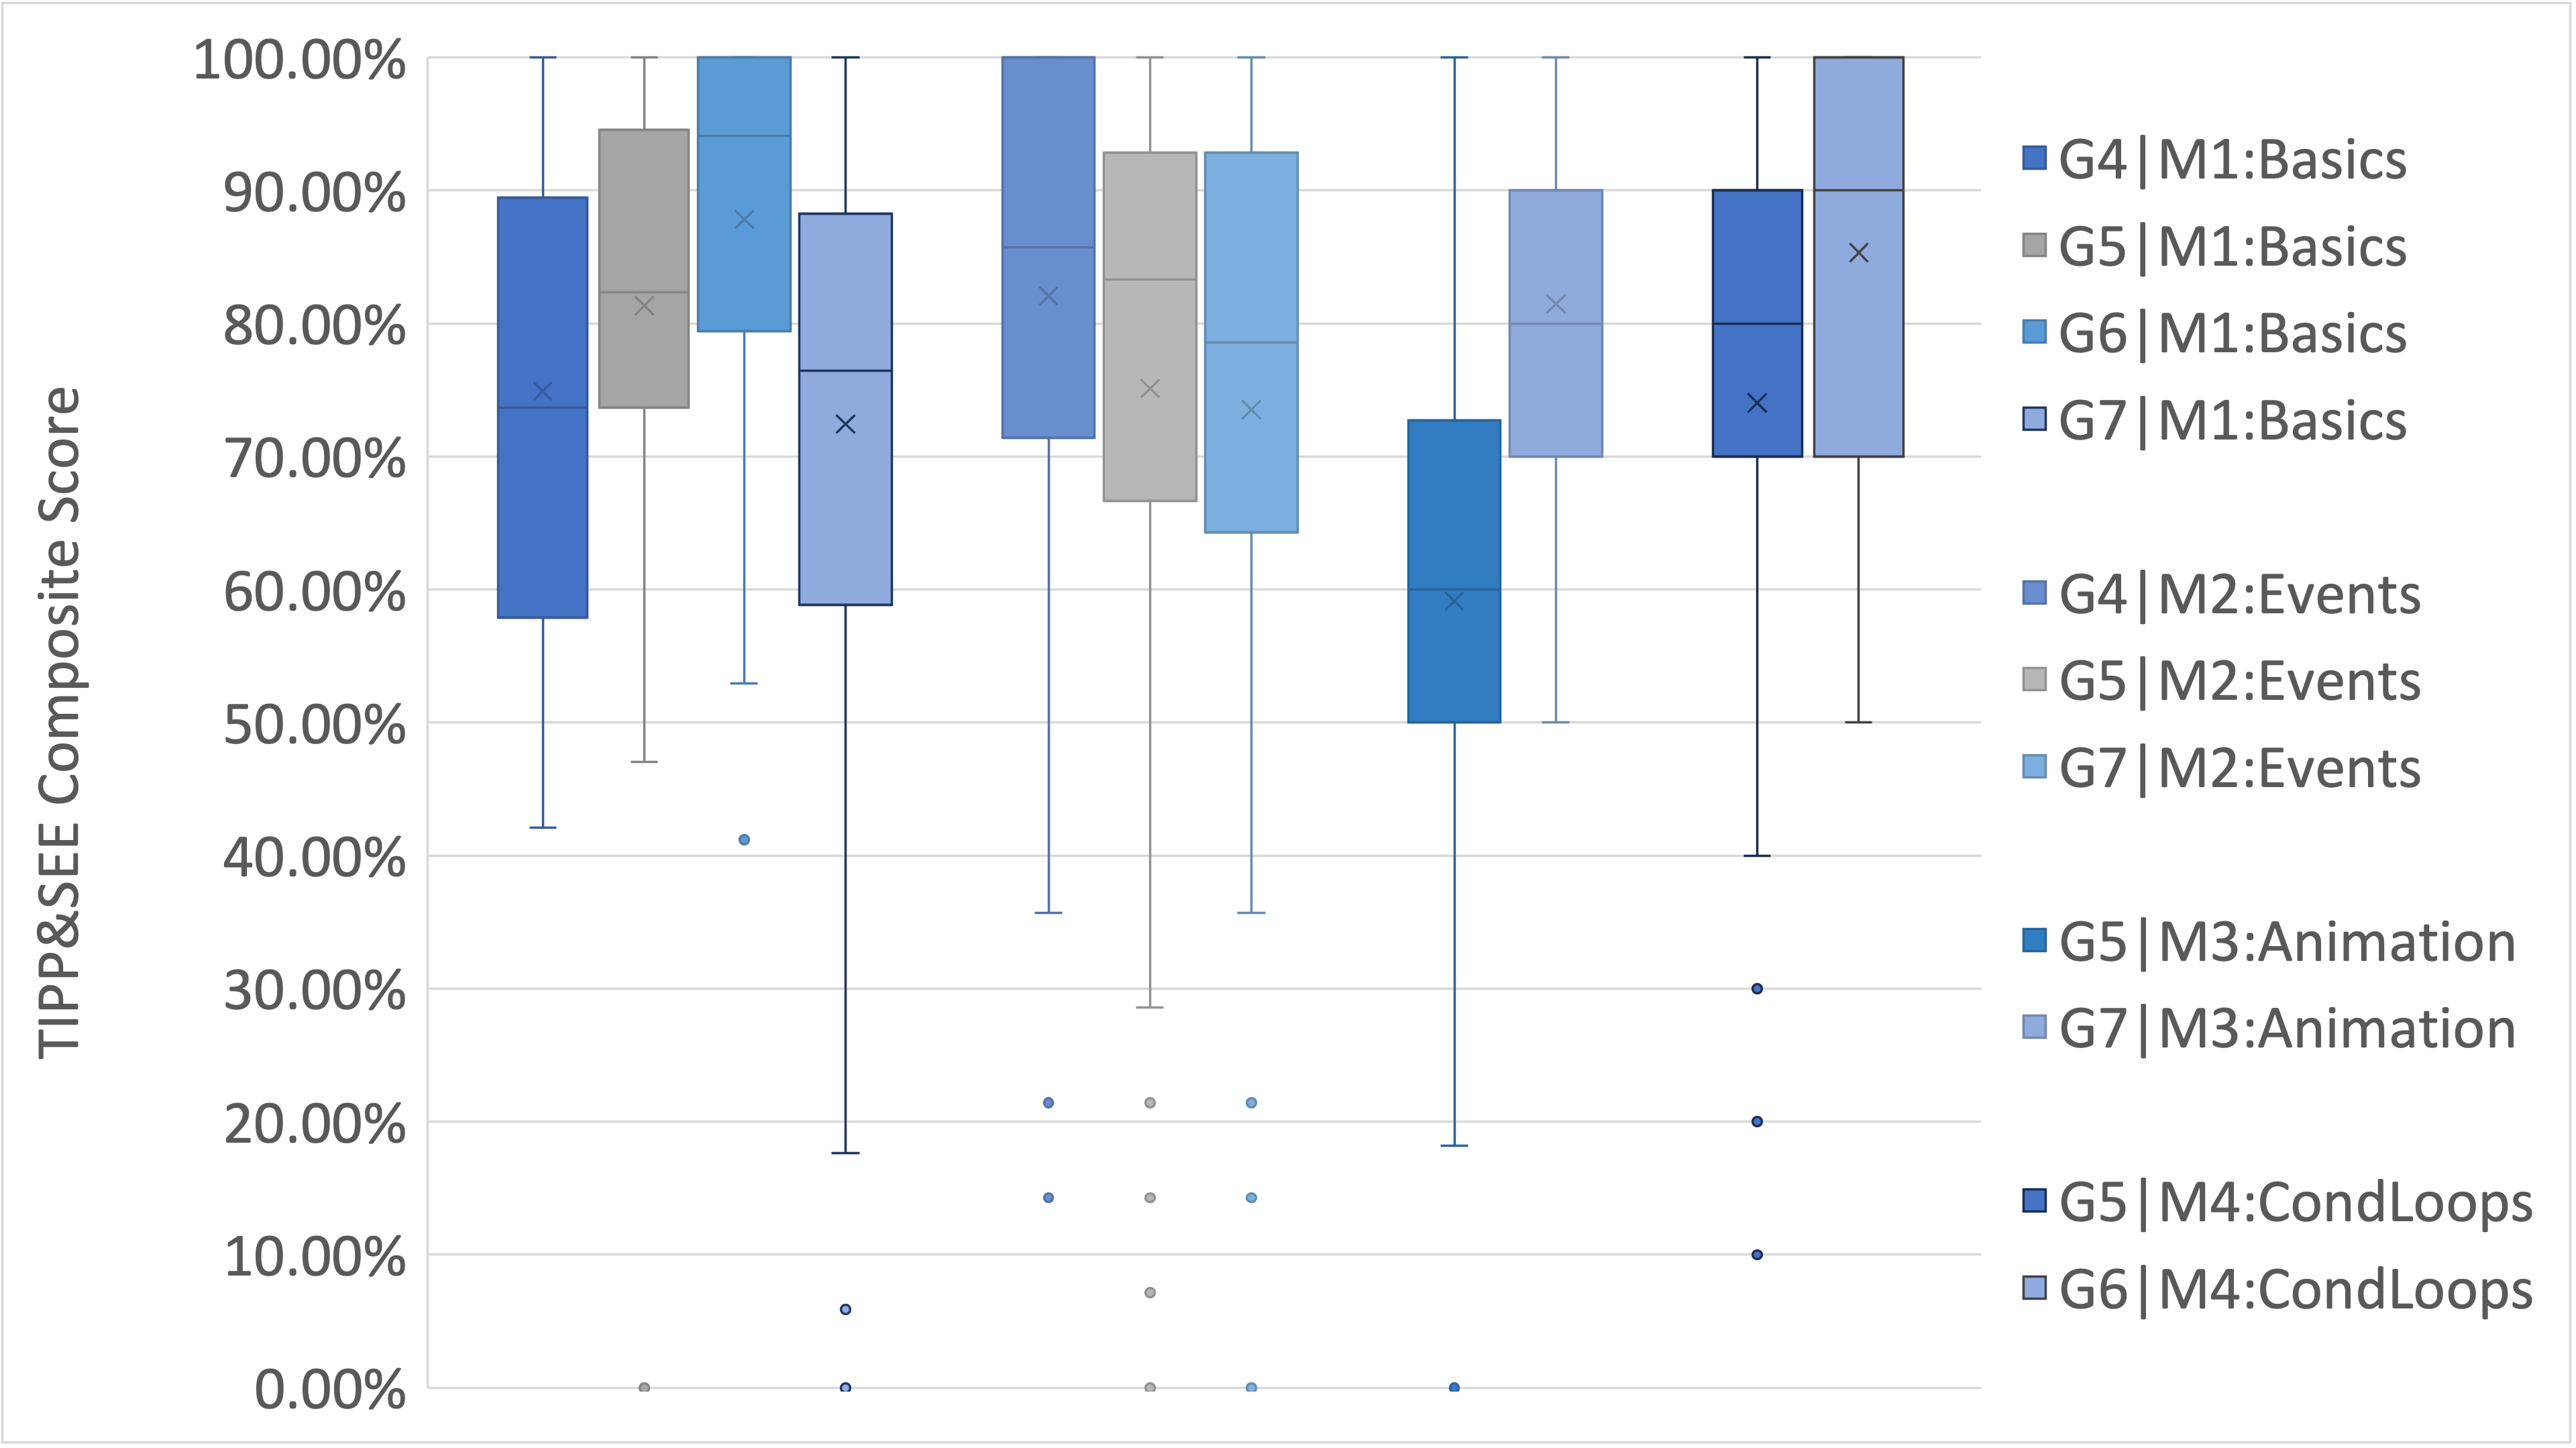
\includegraphics[width=\textwidth]{graphs/Grade.png}}
        \caption{\ts{} Worksheet Composite Scores of Students in Various Middle-School Grade Levels, by \Scratchencore{} Module}
        \label{fig:grade_factors}
    \end{subfigure}
    \hfill
    \begin{subfigure}[t]{0.49\textwidth}
        \raisebox{-\height}{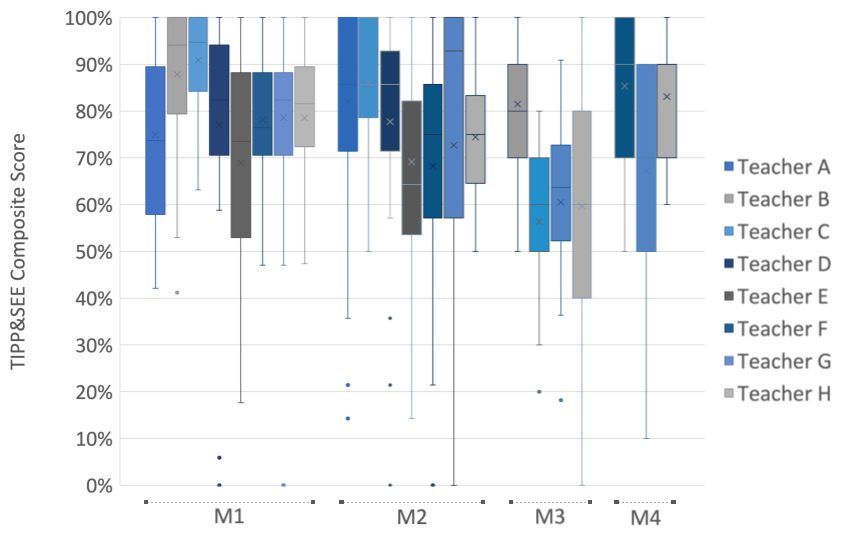
\includegraphics[width=\textwidth]{graphs/Teachers.png}}
        \caption{\ts{} Worksheet Composite Scores of Students with Different Teachers, by \Scratchencore{} Module}
        \label{fig:teacher_factors}
    \end{subfigure}
    \caption{\ts{} Scores Compared Across Classroom-Level Factors (Grade and Teacher)}
    \label{fig:classroom_factors}
\end{figure}

\stepcounter{findingnum}
\textit{Finding \arabic{findingnum}: Grade level was associated with performance for some modules.}

Figure \ref{fig:grade_factors} illustrates the difference in \ts() worksheet performance by grade level. For all modules except M2:Events, grade level was linked to worksheet correctness (M1:Basics:\begin{math}F(3, 255)=6.67, p<.01, \eta^2=.0728; \text{M3:Animation:}\chi=23.79, p<.01, \eta^2=.0747; \text{M4:CondLoops} \chi=4.60, p<.05, \eta^2=.0118\end{math}). Post-hoc comparisons for M1:Basics reveal that 6th graders statistically-significantly out-performed both 4th (\begin{math}p=.0127\end{math}) and 7th graders(\begin{math}p=9.32\times10^{-4}\end{math}), and that 5th graders out-performed 7th graders (\begin{math}p=8.64\times10^{-3}\end{math}). It could be that 7th grade students found this Scratch introduction too easy and were not careful in answering the questions. For M3:Animation, the module with the most difficult content overall, 7th graders performed better than 5th graders (\begin{math}p<.01\end{math}). For M4:CondLoops, 6th graders performed better than 5th graders (\begin{math}p<.05\end{math}). This suggests that some modules may be too difficult or too easy for students in specific grade levels and, therefore, more care needs to be taken in tailoring content to different grade levels.

%For M2:Events, students across all grade levels completed the worksheets with similar correctness M2:Events:(\begin{math} F(2,209)=1.76, p=.175\end{math}). In contrast, for M1:Basics, M3:Animation and M4:CondLoops, grade level was linked to worksheet correctness M1:Basics:(\begin{math}F(3, 255)=6.67, p<.01, \eta^2=.0728; \text{M3:Animation:}\chi=23.79, p<.01, \eta^2=.0747; \text{M4:CondLoops} \chi=4.60, p<.05, \eta^2=.0118\end{math}). Post-hoc comparisons for M1:Basics reveal that 6th graders statistically-significantly out-performed both 4th and 7th graders, and that 5th graders out-performed 7th graders (\begin{math}p<.05\end{math}). It could be that 7th grade students find the material too easy and are not careful in answering the questions. For M3:Animation, 7th graders performed better than 5th graders (\begin{math}p<.01\end{math}). For M4:CondLoops, 6th graders performed better than 5th graders (\begin{math}p<.05\end{math}). This suggests that some modules may be more difficult for students in specific grade levels and, therefore, we may need to develop more support for students in some modules.

\textit{Finding \arabic{findingnum}: Teacher was associated with performance for all modules.}
Performance broken down by teacher is depicted in Figure \ref{fig:teacher_factors}.  For all modules, the teacher was significantly linked to worksheet correctness M1:Basics:(\begin{math} \chi=38.17, p<.01, \eta^2=.104; \text{M2:Events:} \chi=19.27, p<.01, \eta^2=.0442, \text{M3:Animation:} \chi=29.68, p<.01, \eta^2=.0881, \text{M4:CondLoops} \chi=12.63, p<.01, \eta^2=.0350\end{math}). Teachers are likely to implement the curriculum and learning strategies differently. Additional research is needed to better understand how different teaching techniques influence student performance (on \ts{} worksheets as well as learning).


\subsubsection{Student-Related Factors} 
Next we present results considering relevant academic characteristics of students, namely the effect of their previous math and coding experience on their performance with \ts{}.

\stepcounter{findingnum}
 \textit{Finding \arabic{findingnum}: Students using \ts{} with parent-reported mathematics struggles performed equally well to their peers that did not report mathematics struggles on \ts worksheets for some modules, and under-performed compared to their peers in others.}
 
 \begin{figure}
     \centering
    \begin{subfigure}[t]{0.49\textwidth}
        \raisebox{-\height}{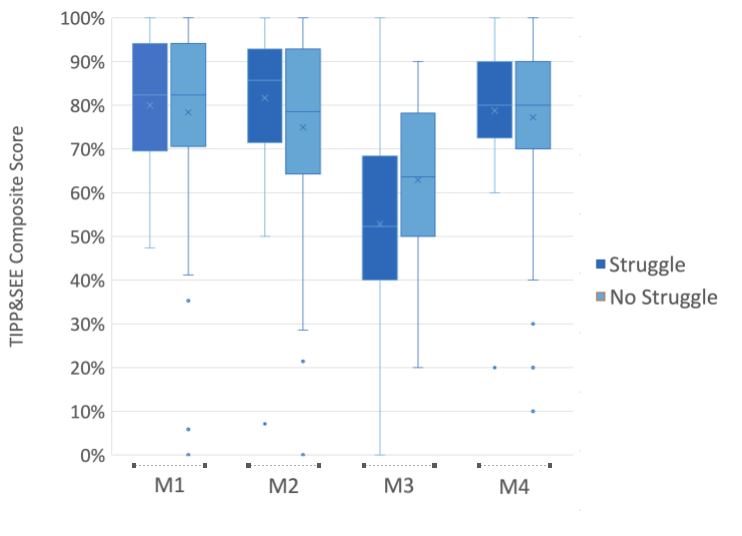
\includegraphics[width=\textwidth]{graphs/Math.png}}
        \caption{\ts{} Worksheet Composite Scores of Students who do and do not Self-Reportedly Struggle on Mathematics Homework, by \Scratchencore{} Module}
        \label{fig:math_struggles}
    \end{subfigure}
    \hfill
    \begin{subfigure}[t]{0.49\textwidth}
        \raisebox{-\height}{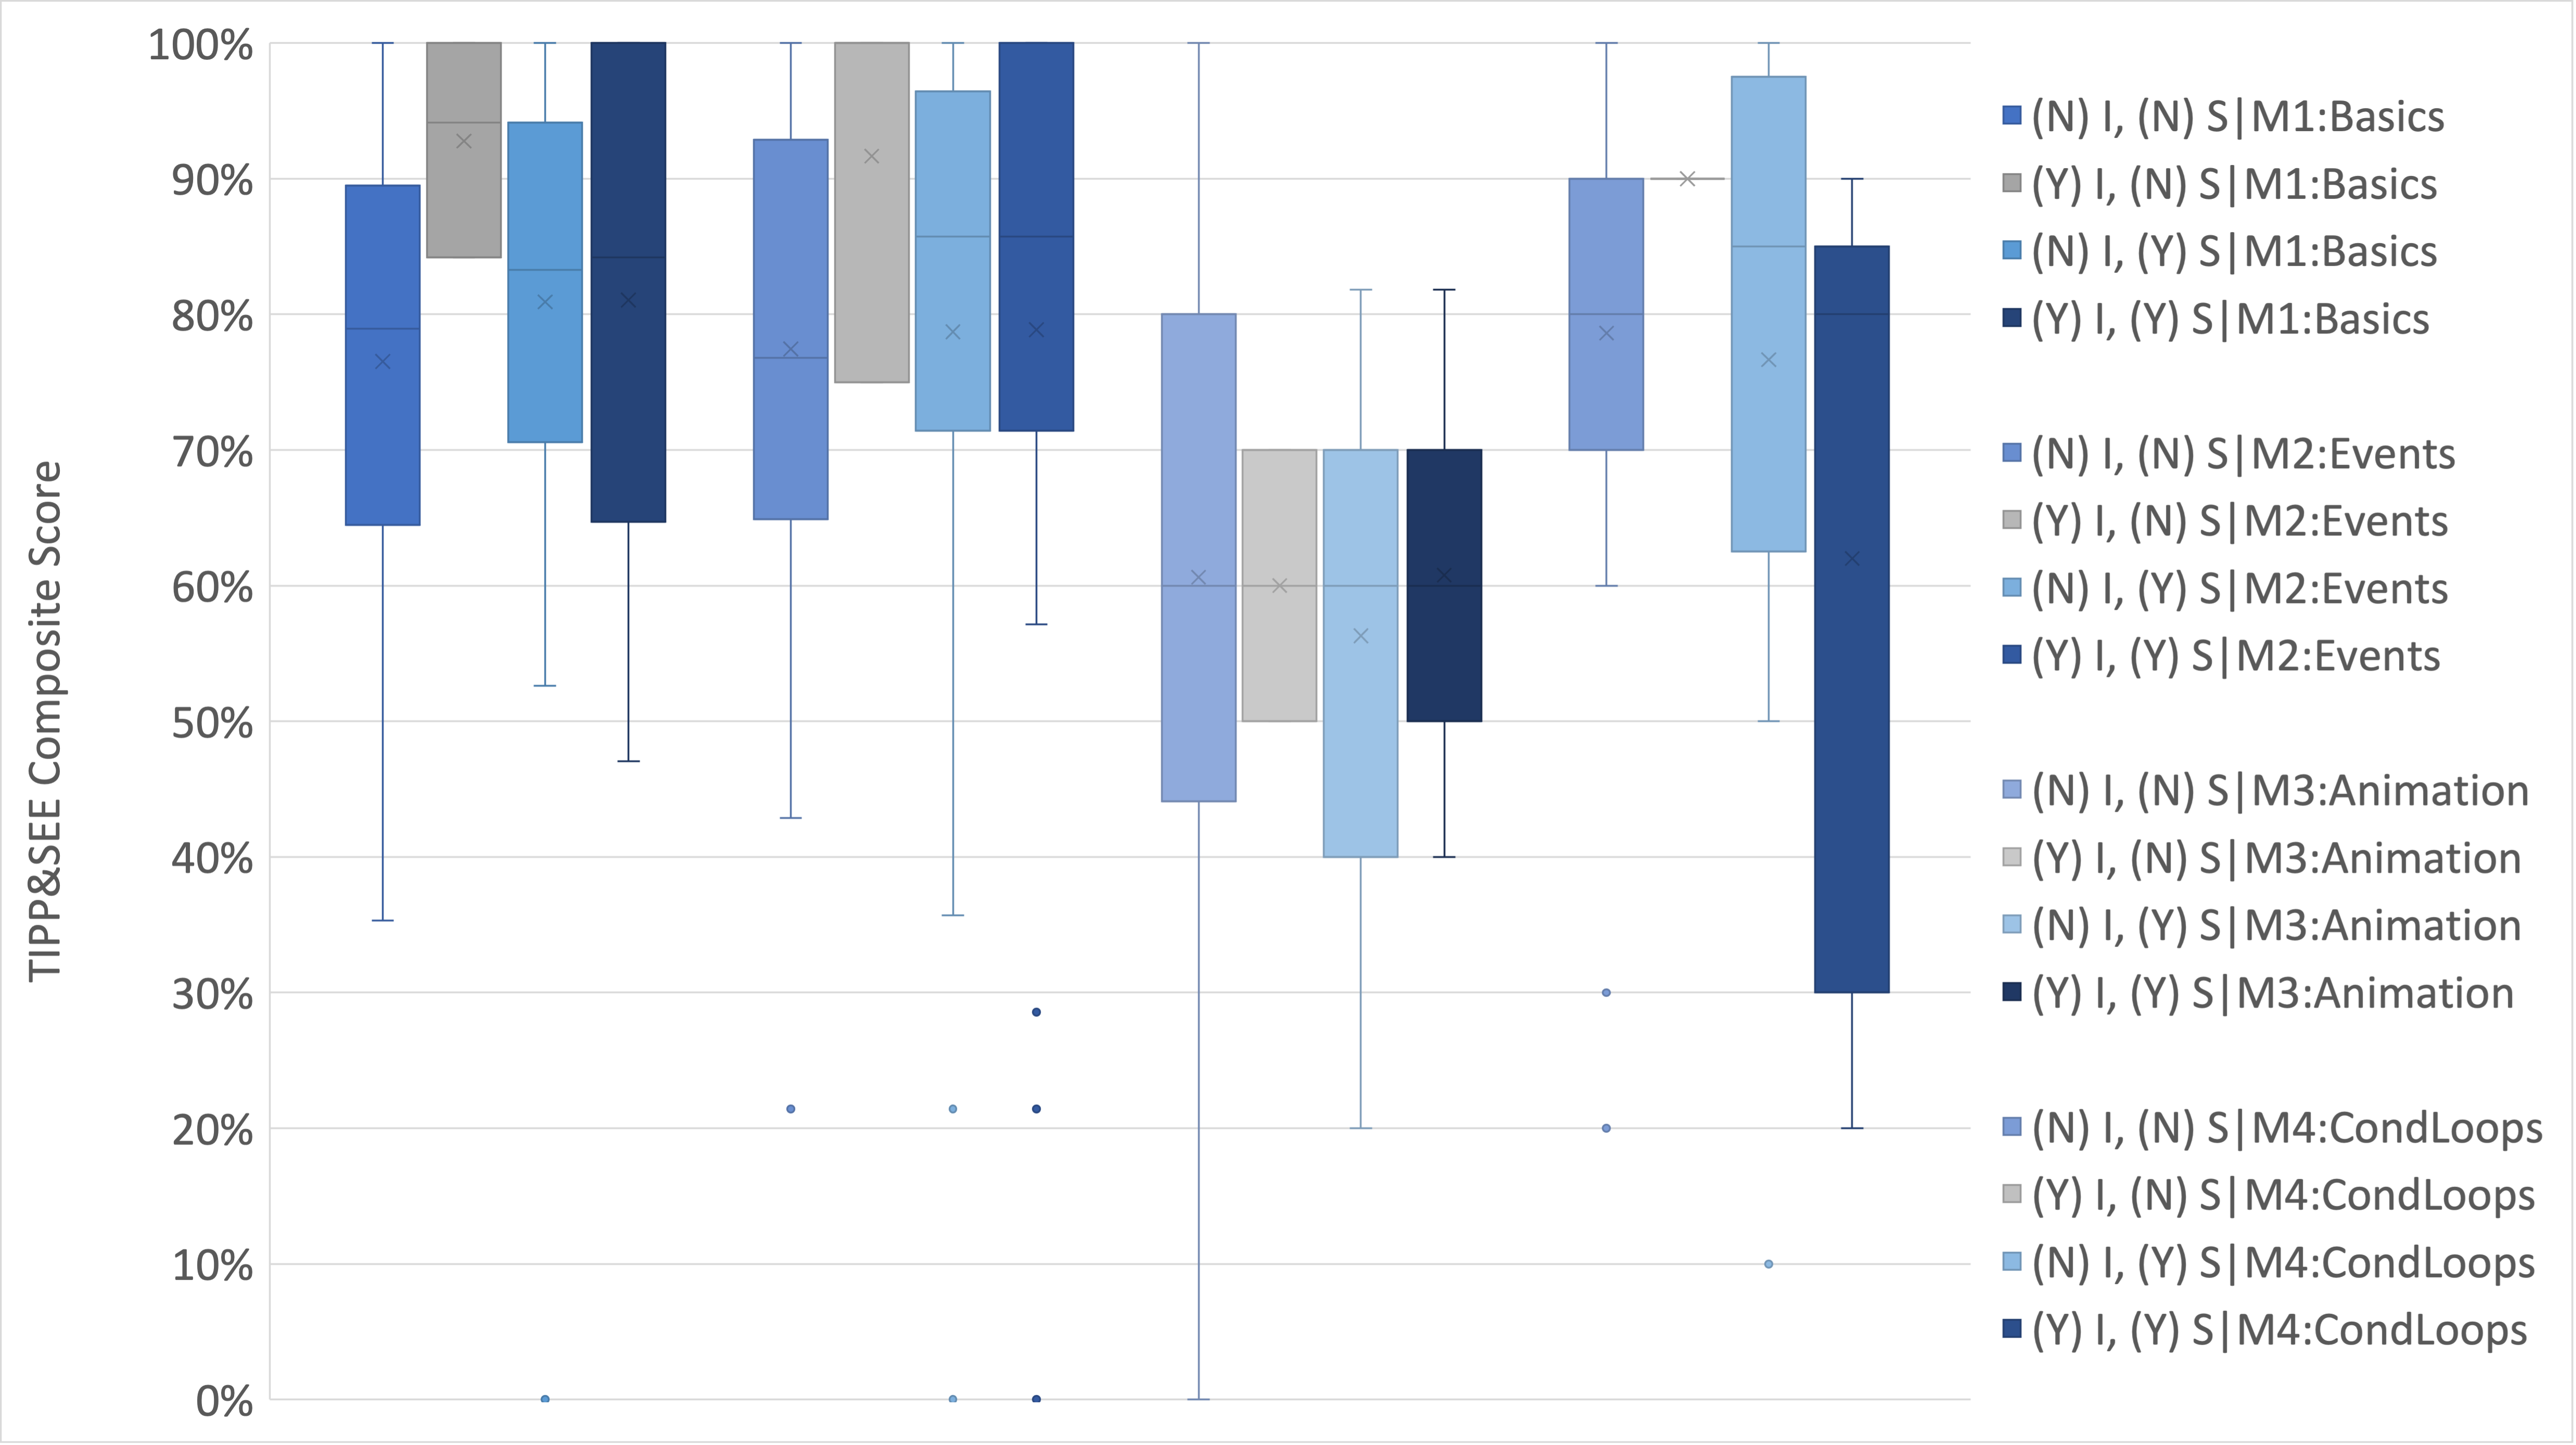
\includegraphics[width=\textwidth]{graphs/Previous_Experience.png}}
    \caption{Average \ts{} Worksheet Composite Scores of Students with Various Combinations of Levels of Informal and In-School Programming Experience, by \Scratchencore{} Module} 
    \label{fig:progexp}
    \end{subfigure}
    \caption{\ts{} Scores Compared Across Levels of Previous STEM Experience}
    \label{fig:math_programming}
\end{figure}

Figure \ref{fig:math_struggles} presents the average composite \ts{} worksheet scores of students whose parents indicated that the student has struggled to complete their mathematics homework in the past compared to those who did not struggle. The average \ts{} composite score for students with mathematics struggle was 73.50\% compared to 73.25\% for students with no reported difficulty. Our statistical analysis showed that there was no significant difference in performance on \ts{} worksheets between students with and without parent-reported struggles in math in M2:Events and M4:CondLoops (\begin{math} F(2,139)=1.23, p=0.295; \text{M4:CondLoops:} \chi=0.00367, p=0.952\end{math}). In contrast, students who struggled with mathematics under-performed on M1:Basics and M3:Animation (M1:Basics:\begin{math} F(2, 147)=3.17, p<.05, \eta^2=.0414; \text{M3:Animation:} \chi=4.09, p<0.05, \eta^2=.0187\end{math}). The modules cover different topics and some topics may require a better understanding of math concepts than others.

\stepcounter{findingnum}
 \textit{Finding \arabic{findingnum}: Students using \ts{} performed equally well on worksheets regardless of their previous experience with programming.}

Figure \ref{fig:progexp} presents the average composite scores of students stratified by their experience with programming in an informal or school setting. While students with only informal experience did slightly better than the others (87.29\% vs 76.34-78.75\%), these differences were not statistically-significant (M1:Basics:\begin{math} \chi=4.94, p=.176; \text{M2:Events:} \chi=4.25, p=.236; \text{M3:Animation:} \chi=.820, p=.235; \text{M4:CondLoops:} \chi=2.19, p=.532\end{math}). These results are promising and indicate that \ts{} is effective in serving as an equitable learning strategy despite students' previous experiences as reported by their parents.

\subsubsection{Question-Related Factors} 
We now delve deeper into individual question differences. The goal was to identify individual questions on which students performed worse than others, identify potential factors that distinguish the poorly-performing from well-performing questions, and perform statistical tests to determine whether that factor correlated with performance. Here, we present the 2 factors we identified that were statistically correlated with differences in performance.

\stepcounter{findingnum}
\textit{Finding \arabic{findingnum}: Students are more likely to answer questions and to do so accurately when the block or concept in question has a real-world, common-sense, everyday interpretation.}

%Figure \ref{fig:everyday_school} illustrates the differences in answer correctness and answer rate for \ts{} worksheet questions when divided by whether they were asking students about a concept which matched with its real-world interpretation (``Everyday True Positive''), did not match with its real-world interpretation (``Everyday False Positive''), or did not have a straightforward real-world interpretation to begin with and relied primarily on knowledge gained in school settings (``Mathematics''). The figure displays the percent of each response type (correct, incorrect, and blank) in each category. We found a statistically-significant association between response type and the type of knowledge used for a concept (\begin{math}\chi=55.89, p<.01\end{math}).


Figure \ref{fig:e_ef_s} illustrates the differences in answer rate for ``Predict'' and ``Explore''\ts{} worksheet questions when categorized by whether they were asking students about a concept which matched with its real-world interpretation (``Everyday True Positive''), did not match with its real-world interpretation (``Everyday False Positive''), or did not have a straightforward real-world interpretation to begin with and relied primarily on knowledge about the Cartesian system (``X-Y Coordinate''). The figure displays the percent of each response type (correct, incorrect, and blank) in each category. Aggregating both ``Predict'' and ``Observe'' questions, we found a statistically-significant association between response type and the type of knowledge used for a concept (\begin{math}\chi=23.39, p<.01\end{math}). This trend still held true when ``Predict'' and ``Explore'' questions were analyzed separately (``Predict'':\begin{math}\chi=14.604, p<.01\end{math}, ``Explore'':\begin{math}\chi=15.173, p<.01\end{math}). ``Everyday True Positive'' questions were answered correctly 76.01\% and whereas only 65.38\% of ``Everyday False Positive'' questions and 69.16\% of ``Mathematics'' questions were answered correctly. Furthermore, students only left 9.26\% of ``Everyday True Positive'' questions blank while leaving 19.23\% of ``Everyday False Positive'' questions blank and 12.85\% of ``X-Y Coordinate'' questions blank. 



%Additionally, students answered more ``Mathematics'' questions incorrectly (17.91\%) than ``Everyday True Positive'' (15.23\%) and ``Everyday False Positive'' (9.93\%) questions.
%This data shows that questions testing blocks or concepts that require knowledge about the Cartesian coordinate system are the most likely to be answered incorrectly by middle-grade students when engaging with the \ts{} learning strategy and questions testing blocks or concepts that match their everyday common sense interpretation are the most likely to be answered and answered correctly. This behavior may occur because students are associating those blocks or concepts with concepts they have learned in other subjects. Therefore, students may be less comfortable blocks that ask students to use the coordinate system. 

%This data shows that questions testing blocks or concepts that are connected to a mathematics-knowledge meaning are the most likely to be skipped or answered incorrectly by middle-grade students when engaging with the \ts{} learning strategy and questions testing blocks or concepts that match their everyday common sense interpretation are the most likely to be answered. This behavior may occur because students are associating those blocks or concepts with concepts they have learned in other subjects. Therefore, students who may be less comfortable with certain blocks or concepts, such as variables or blocks that ask students to use the coordinate system.

% this is the ``so what'' but maybe it belongs in the discussion? I put it both places to decide where it goes better:

%\ts{} and \Scratchencore were created and this study was conducted in order to provide equitable access to intermediate CS education to middle-grade students. In order to do so, it is important to understand if the \ts{} worksheets impacts student success on theoretical and abstract concepts. In finding 0, we demonstrate that parent-reported previous coursework in programming and mathematics does not impact student engagement or success. In this finding, however, we show that the \ts{} worksheets that include concepts from previous coursework in mathematics and CS do impact student engagement as they are the most frequently skipped and the most frequently answered incorrectly. This may be indicative of middle-school students' perceptions of the relevance of other coursework to their CS education. Further research could involve asking students if they perceived the ``Mathematics'' questions as implying that their performance in their other coursework was relevant to their success in their CS course work. This pre-judgement may cause students to simply not answer the question, if they feel it appears to require knowledge from other coursework.

\stepcounter{findingnum}
\textit{Finding \arabic{findingnum}: The position of a question within a section was associated with students' attempt and correctness rates.} 

\begin{figure}
     \centering
    \begin{subfigure}[t]{0.49\textwidth}
        \raisebox{-\height}{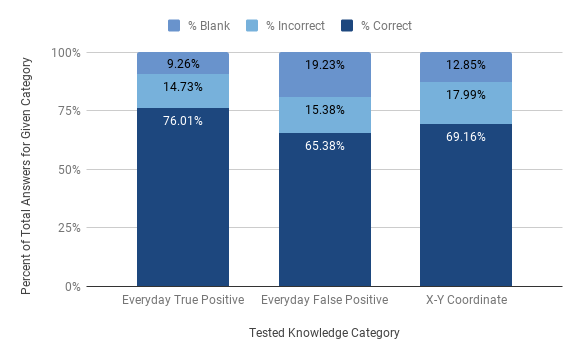
\includegraphics[width=\textwidth]{graphs/E_EF_S.png}}
        \caption{Student Performance on \ts{} Worksheets by ``Everyday True Positive'', ``Everyday False Positive'', and ``X-Y Coordinate' Knowledge Categorization}
        \label{fig:e_ef_s}
    \end{subfigure}
    \hfill
    \begin{subfigure}[t]{0.49\textwidth}
        \raisebox{-\height}{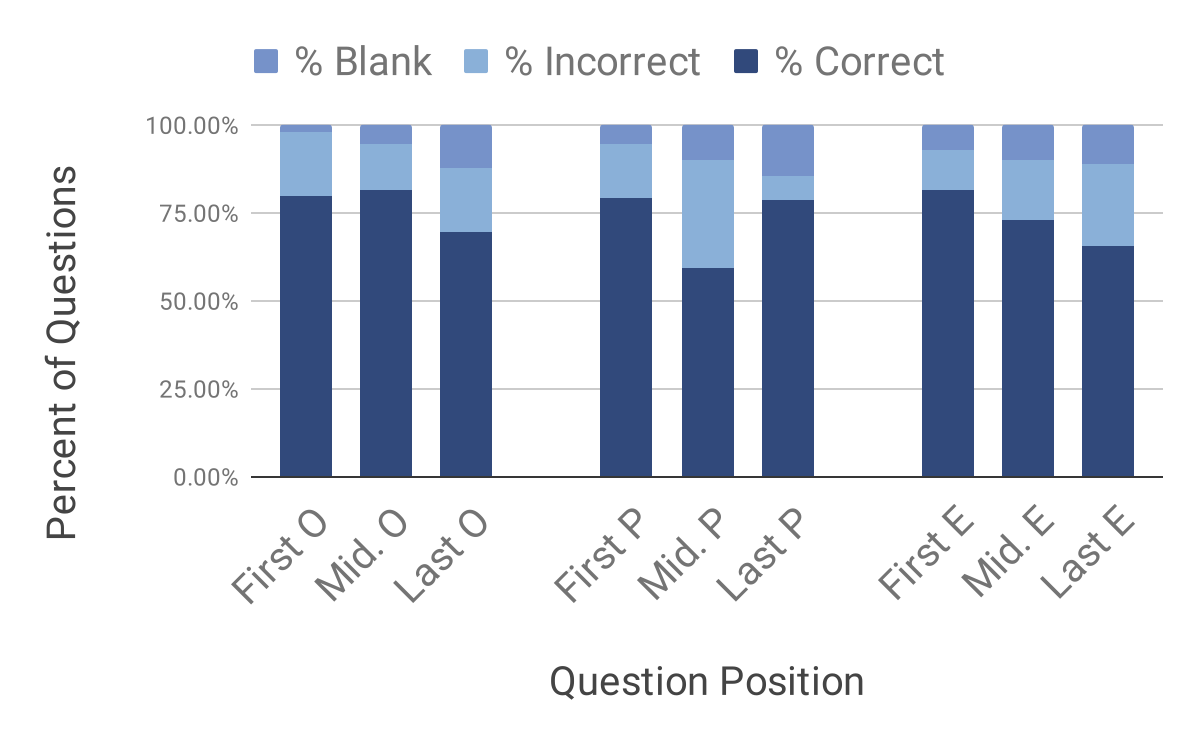
\includegraphics[width=\textwidth]{graphs/Position.png}}
    \caption{Question Performance by Question Position in Observe (O), Predict (P), and Explore (E) sections on \ts{} Worksheets} 
    \label{fig:pos}
    \end{subfigure}
    \caption{Student Performance Compared Across Question Position and Question Knowledge-type}
    \label{fig:position_es}
\end{figure}

In Figure ~\ref{fig:position_es}, 3 lines are shown: correct (percent of attempted questions answered correctly), incorrect (percent of attempted questions answered incorrectly), and blank (percent of questions not attempted) as a function of the position of a question within a section of the worksheet, being the first, middle or last question in a given section. The students tended to attempt fewer questions as they progressed through each section, and the percentage of correct answers decreased through each section (\begin{math}\chi=76.06, p<.01\end{math}). There was similar percentage of incorrect answers from the first to the last question in the sections.

In the ``Observe'' section, there were not any noticeable trends in the percentage of correct or incorrect answers from the first question to the last question. However, there was an increase in blank answers from the first to the last question (first: 5.31\%, middle: 9.81\%, last: 14.50\%). Similarly, we did not observe any noticeable trends in the percentage of correct or incorrect answers in the ``Predict'' sections. However, there was an increase from 5.31\% to 14.50\% in blank questions for the questions in the ``Predict'' section.

The position of a question had the strongest impact on answer correctness in the ``Explore'' section. For this section, the final section of the worksheets, the percentage of correct answers changed from 81.22\% on the first question to 65.83\% on the last question. In this section, students incorrectly answered twice as many questions at the end of the section as they did at the start of the section (11.64\% to 23.28\%). Additionally, there was an increase in blank answers (first: 7.16\%, middle: 10.00\%, last: 10.94\%).

Despite there being no clear trend in incorrectness/correctness with respect to question position in the individual ``Observe'' and ``Predict'' sections, the rate of blankness rose steadily from the first to the middle through the last question of all 3 sections. These findings may be due to the students becoming tired of answering questions from the first to last question in the sections.%there was an decrease in the average percentage of correct answers from the first to last question in all sections. Additionally, 

\section{Discussion}
\label{sec:discussion}
In this section, we place our findings in larger context. We first compare to previously-published work - on a different grade level (4th grade only) and a different curriculum - in order to understand what may be a trend related to \ts{} itself vs. what my be correlated with a specific grade level or implementation. Second, we look at findings that were unique to this study to relate them to potential reasons beyond this study.

\subsection{Relating to Prior Work}
\label{sec:compare}
Here we compare the results in our study with the results of one previously-published study on
student behavior using \ts{} \cite{franklin2020exploring}. There are 2 major differences between their study and our study. First, their study consisted of only 4th-grade classrooms, many of which were bilingual. Second, they used a different curriculum. The curriculum had several differences, including different projects, different formatting of their \ts{} worksheets, different individual questions on the \ts{} worksheets, and slightly different content (no coverage of conditional loops). Our goal is to gain insight into what findings based on the use of \ts{} hold across curricula and age groups.

To perform this comparison, we focus on the findings in both papers and compare which ones are both present and whether they align or are contradictory. 

\begin{table}
    \centering
%\includegraphics[width=\textwidth]{class_nums.png}
\begin{tabular}{| c | c |} 
      \hline
Comparison & Finding \\ \hline
Similar & Students completed and correctly answered ``Observe'' questions the most \\ \hline
Similar & Students leave the most blank answers in ``Explore'' questions \\ \hline
Dissimilar & Our study's students had higher \textit{accuracy} on ``Explore'' questions than prior study \\ \hline
Similar & Completion and accuracy rates differ by teacher \\ \hline
Similar & \ts{} completion and accuracy are not correlated with project completion \\ \hline



%\multicolumn{3}{|l|}{Total} & 317 \\ \hline
   \end{tabular}

    \caption{Findings Comparison}
    \label{tab:table2}
\end{table}


\textbf{Observe, Predict, and Explore.} 
In both studies, students answered ``Observe'' questions most often and most accurately. In addition, ``Explore'' questions were answered incorrectly the most often. That these trends hold across both studies suggests that these trends are likely inherent in these types of questions. 

Thinking about the 3 types of questions, this is perhaps not surprising, because ``Observe'' questions ask about what they see in a running program, which is analogous to merely using a program. ``Predict'' and ``Explore'' questions are inherently more difficult but for different reasons. ``Predict'' questions are more cognitively difficult, asking about which block performed which action. ``Explore'' questions, on the other hand, require students to make specific changes and compare the output before the change to after the change. This requires that the student actually perform the change properly and remember the prior output accurately. Students may just attempt to guess what will happen if they do not want to go through the work of changing it.

%One of our findings was that students answered ``Observe'' questions the most and were more correct on these questions than ``Predict'' and ``Explore'' questions. Students were least likely to attempt ``Predict'' questions. Although ``Explore'' questions were answered more than ``Predict'' questions, ``Explore'' questions had the greatest percentage of incorrect answers. Comparing our findings with previous work, we find that both previous work (with 4th grade students) and our work (with 4th-7th grade students) revealed that students who use \ts{} completed and correctly answered ``Observe'' questions the most \cite{franklin2020exploring}. In contrast, students in our data set answered ``Explore'' questions the least but also answered them more correctly than students in the prior work \cite{franklin2020exploring}.

%The ``Observe'' questions require students to participate in the learning process, but do not require the cognitive engagement of predicting the outcome, or exploring the effects of changing the code after the fact. This may provide insight into why the ``Observe'' questions were not only answered more often than the other 2 categories, but also were answered correctly more often. The ``Observe'' questions may require less of a cognitive leap than ``Predict'' or ``Explore'' questions, which require more insight into the functionality of the operations in the code. This may also be why our findings are consistent with previous findings about ``Observe'' questions.

It is also interesting that the ``Explore'' questions were attempted more often in this work than the ``Predict'' questions, which may provide insight into the student learning process. There is perhaps less of a cognitive barrier to changing the code and inspecting the behavior (``Explore'') than predicting the outcome without the opportunity to explore the effects of the code change (``Predict''). This may also explain why students answered more ``Explore'' questions incorrectly than the other questions. We believe that our current results differ from previous results \cite{franklin2020exploring} because our dataset includes students from 4th through 7th grade. The older students may become tired less easily and also complete the work more quickly. The younger students in the previous study may have also focused on the coding part of the ``Explore'' section and forgotten to complete the worksheet part of the section. These findings suggest a need for more guidance and support for the ``Predict'' and ``Explore'' questions. Specifically, we need to encourage students to attempt ``Predict'' questions more. For ``Explore'' questions, further examination is needed to see why their answers are incorrect more often.

%\textbf{Module and Teacher.} %We found that across 2 modules, student performance with \ts{} did not significantly vary based on grade level. However, their performance did vary between modules and between teachers. Some of these findings are consistent with previous findings \cite{franklin2020exploring}. Because of \ts{}'s similar effectiveness across grade levels in middle-grade students, it may be particularly adept for environments where only 1 teacher is responsible for teaching computing concepts to students from several different grades. Franklin et al. discovered that across grade levels, students were able to complete the activities \cite{franklin2020analysis}. We analyzed the students' performance at various grade levels. First, we found that 6th graders differed from 4th and 7th in M1:Basics. We believe that this may be the case because the 6th grade teachers may have been more experienced. We also found that 7th graders differed from 5th graders in M3:Animation and 6th graders differed from 5th graders in M4:CondLoops. This suggests that 5th graders may need more support in some modules and that even though students in all grade levels may be able to complete \ts{}, they may still struggle with answering questions correctly. Tied to that finding is our finding that performance differed between modules. M3:Animation had the lowest average \ts{} scores. This further supports the idea that modules vary in difficulty and students also need varying support. 

%Similar to this study, Franklin et al. found that the completion rates of \ts{} differed based on teacher \cite{franklin2020analysis}. \cite{franklin2020analysis} hypothesized that the flexibility of the curriculum could be a cause of this finding. %This could also explain our finding of differences in scores between teachers. 
%Students' scores could be affected by how individual teachers choose to implement the curriculum. %Based on these results, we believe that \ts{} should be adapted for varying grade levels in some modules. 
%We also need to further investigate how the teachers are implementing \Scratchencore{} and \ts{} to understand what the most effective practices are and encourage other teachers to follow those practices. 

\textbf{\ts{} and Projects.} Similar to findings from previous work \cite{franklin2020exploring}, our analysis revealed the correlation between \ts{} worksheet score and project score was weak. 

When we take 2 findings together (teacher influences worksheet completion and accuracy and worksheets do not correlate with project score) and triangulate that with our observation field notes, a possible theory emerges. 
 Different teachers place different emphasis on accurate completion of the worksheet. One teacher, for example, had students check off their completed worksheet with the teacher. If it was not correct or complete, the teacher required that they go back and try again until it was correct. That teacher did not allow students to continue to modify without accurately completing the \ts{}. Another teacher, on the other hand, went over the worksheet with the entire class before moving on. Both techniques are based on sound pedagogical principles - they wanted to make sure students had some basic understanding of the \ts{} exercise prior to moving on. In both classrooms, we would expect to see higher completion and accuracy than other classrooms. In addition, the first teacher's technique may lead to better learning since students needed to figure out the answers themselves rather than being told by the teacher later. Because teachers varied in how they treated the worksheet, it is not unexpected that the completion and accuracy differed. In addition, these differences could also affect the correlation with understand and/or project performance.
 
 \subsection{Unique Findings}
 We now discuss findings that were not in prior work in order to explore possible explanations and implications.

\textbf{``Everyday True Positive'', ``Everyday False Positive'', and ``X-Y Coordinate''.} We found a significant difference in students' likeliness to answer, and answer accurately, questions that pertain to blocks or concepts that can be interpreted based on real-world, everyday concepts. In other words, \ts{} worksheet questions that involved x-y coordinates and questions concerning blocks or concepts that a have a real world, everyday interpretation that does not match with their role in Scratch (``Everyday False Positive'' questions) impact student engagement as ``X-Y Coordinate'' questions are answered incorrectly the most often and ``Everyday False Positive'' are the most frequently skipped and the least frequently answered correctly. 

In the state where we collected data, the coordinate system is not covered until 5th grade. Additionally, coverage of a concept does not ensure that students understand them. Given these facts, we theorize that the students who struggled in these questions were ones that have not learned the coordinate system yet to the point where they are comfortable, confident, and accurate in their use of it. Further research is required to learn if this is the case. If so, we should offer additional support for learning blocks and concepts that require mathematical knowledge beyond students' mathematical instruction.
 
``Everyday False Postive'' questions can also be confusing to students. They may interpret the Scratch blocks using their knowledge of what the words mean in everyday language. For example, asking the students to change the value in a \texttt{move} block and then observing how that changed a sprite's behavior, or what the \texttt{wait () seconds} block does. It is important that teachers recognize the differences between everyday interpretations and Scratch interpretations and explicitly teach what it means in Scratch.

%Encouragingly, if the blocks or concepts tested do have a real world, everyday interpretation that does not match with their role in Scratch, students are still able to answer the question with comparable correctness to questions where the everyday interpretation does match. This suggests that students are able to separate the blocks and concepts from everyday concepts and learn programming.

\textbf{Question Location}. Students tended to attempt fewer questions, and answer them with decreasing accuracy, as they progressed through the worksheet. This was most dramatic in the final section of the worksheet. These findings could be due to cognitive fatigue \cite{sievertsen2016cognitive}. That is, students may become fatigued from answering questions from the beginning of a section to the end of a section, and from the beginning of a worksheet to the end of a worksheet.  In order for students to have the desired learning outcomes, we must further understand the sources of worksheet fatigue and work to mitigate these effects where possible. This might entail worksheets of varying length and providing an option to pause and restart a given worksheet at a later time, along with a study to see if such methods improve learning fatigue.

\textbf{Math and Programming.} There were not any differences in student outcomes based on previous experience with programming, indicating \ts{} may have served effectively as an equitable factor across differences in parent-reported previous programming experience. This further bolsters the argument to use \ts{} in diverse classroom environments where students have varying levels of programming experience and are not able to receive highly personalized attention from educators. 

Results were more mixed with respect to parent-reported mathematics struggles, where students with math struggles performing similarly in some modules and under-performing in other modules. This echoes prior work that has found differences in CS assessment performance %between 4th grade students ~\cite{salac2020comprehending} and 
middle-school students \cite{grover2016factors,qian2016correlates} of different math levels, with differences becoming more prevalent in more advanced CT concepts. However, we do have to keep in mind that our data was collected from parental reports instead of more objective assessments. Due to \ts{}'s abilities to support students regardless of prior programming experience and support students who struggle with mathematics in some modules, \ts{} should be used with middle-grade students. However, we should increase the support in modules where \ts{} was unable to equalize students who struggle with math with students who do not.

\textbf{Module and Teacher.} We found that across 2 modules, student performance with \ts{} did not significantly vary based on grade level. However, their performance did vary between modules and between teachers. Because of \ts{}'s similar effectiveness across grade levels in middle-grade students, it may be particularly adept for environments where only one teacher is responsible for teaching computing concepts to students from several different grades. 

We also analyzed the students' performance at various grade levels. First, we found that 6th graders differed from 4th and 7th in M1:Basics. We believe that this may be the case because the 6th grade teachers may have been more experienced. We also found that 7th graders differed from 5th graders in M3:Animation and 6th graders differed from 5th graders in M4:CondLoops. This suggests that 5th graders may need more support in some modules and that even though students in all grade levels may be able to complete \ts{}, they may still struggle with answering questions correctly. Tied to that finding is our finding that performance differed between modules. M3:Animation had the lowest average \ts{} scores. This further supports the idea that modules vary in difficulty and students also need varying support. 

%Similar to this study, Franklin et al. found that the completion rates of \ts{} differed based on teacher \cite{franklin2020analysis}. \cite{franklin2020analysis} hypothesized that the flexibility of the curriculum could be a cause of this finding. %This could also explain our finding of differences in scores between teachers. 
%Students' scores could be affected by how individual teachers choose to implement the curriculum. %Based on these results, we believe that \ts{} should be adapted for varying grade levels in some modules. 
%We also need to further investigate how the teachers are implementing \Scratchencore{} and \ts{} to understand what the most effective practices are and encourage other teachers to follow those practices. 

%This result seems to contradict our result about ``Everyday'' compared to ``Mathematics'' interpretation. Since the questions labeled as ``Mathematics'' questions were about the coordinate system, it does not represent all of the concepts students from 4th to 7th grade learn in math. Therefore, students, especially older students, may struggle with mathematics concepts that are unrelated to the Scratch concepts learned in the first 4 modules of \Scratchencore{}; this suggests that our results are consistent with each other.

\section{Limitations}
\label{sec:limits}
% Some of the findings may be more significant for certain groups and certain classes than others and further study would be needed to identify these attributes of the trends. It would be worth investigating how these trends correlate across classroom size, gender, grade level, and specific teacher.
The data collection was interrupted by the COVID-19 pandemic and the subsequent switch to online learning. Classroom \Scratchencore{} instruction ended in many cases when classes unexpectedly switched to an online format. While the number of student-presented questions and answers overall is large, the size of a given class or the sample of students given a certain worksheet varied, as different classes completed varying numbers of modules, with fewer classes completing Modules 3 and 4. Additionally, for our first 4 modules, which were the modules we analyzed, the only blocks we covered that required mathematics knowledge are blocks that include using the x-y coordinate system. Future research should investigate other blocks and concepts that can be interpreted differently in subjects outside of CS.%Additionally, future work could include classroom observations, student interviews, or teacher interviews, which may provide insights into some of the findings in this paper, as differences in teaching style might have influenced student engagement with the \ts{} worksheet and further analysis into student perspectives could provide insight for our findings. 
Finally, there are limitations involved in the demographic survey in which parents reported if their student struggled to complete their mathematics homework or if they have experience in programming. Parent answers may be exaggerated, the parents may feel embarrassed to reveal if their student struggles in school, and students may feel embarrassed to reveal to their parents if they struggle in school.

\section{Conclusions}
\label{sec:conclusions}
As CS education is provided to larger quantities and diverse audiences of middle-school students, it is important that we closely examine instructional methods for their use across several grades. In this paper, we explore the \ts{} strategy and its enactment in \Scratchencore. We find that, for the most part, the trends observed at the 4th-grade level in a different curriculum held with this middle-school implementation: students complete ``Observe'' questions most often and accurately, teachers are correlated with worksheet performance, and worksheet performance is not correlated with project performance. This study also had additional findings, such as that students' prior experience with programming had no effect on worksheet performance, and math struggles only affected performance for some modules. Finally, students completed more often and with more accuracy questions about Scratch blocks that have a meaning in Scratch similar to the way a student might interpret that block's meaning according to an every-day interpretation than questions referencing x-y coordinate systems and questions that have a meaning in Scratch that is not similar to the way a student may interpret that block's meaning according to an every-day interpretation. We also discovered that students lose engagement and accuracy as they progress toward the end of a \ts{} worksheet. %These results provide insight into how and where \ts{} is most effective for middle-grade students and how we can increase our support for these students.

%Our analysis reveals that the \umc pedagogical approach%, as enacted through the \Scratchencore{}, provided students a productive balance between structure and open-ended exploration. During open-ended tasks, many students followed guidance in reinforcing new knowledge by utilizing blocks they had just learned. They also explored new blocks not formally introduced, as well as combined existing blocks in new ways. At the same time, students also took advantage of the open-endedness afforded by the Create tasks to explore new blocks as well as to personalize backgrounds, sprites, and narratives to take ownership of their projects and express themselves creatively. Collectively, this work shows one way forward to incorporate the powerful ideas of constructionism learning into the constraints of classrooms, providing one potential path out of the Play Paradox. In doing so, this work helps provide guidance as to one productive way to help bring computing to all learners.

\section{Acknowledgements}
\label{sec:ack}
We would like to thank the teachers and students who piloted \Scratchencore{}. This material is based upon work supported by [Blinded for review] %the National Science Foundation under Grant No. 1738758. 
\hide{}

\bibliographystyle{ACM-Reference-Format}
\balance
\bibliography{ref}

%\printbibliography

\end{document}




